\chapter{The ATLAS Detector}

\label{ch:atlas}
% --------------------------------------------------------------------------------

The four major \ac{LHC} experiments at \ac{CERN} seek to use the never before matched energies and luminosities of the new collider to explore the boundaries of particle physics and to gain insight into the fundamental forces of nature.
Two of these experiments, \ac{ATLAS} and \ac{CMS}, are general purpose detectors that seek to measure a variety of processes in the up to 14 \TeV proton-proton collisions that occur as much as 40 million times per second at the \ac{LHC} at the design luminosity of $10^{34}$ \lcms. 
\ac{ATLAS} employs a hermetic detector design, one which encloses the particle collisions as completely as possible with detecting elements, that allows it to study a wide range of physics from \ac{SM} and Higgs measurements to searches for new physics in models like \acl{SUSY}~\cite{atlas_experiment}.

Accomodating this wide variety of goals is a challenge for the design of the detector.
The wide range of energies involved requires high measurement precision over several orders of magnitude and the ability to measure a variety of particle types.
At the time of the construction of \ac{ATLAS}, the Higgs boson had yet to be discovered, but the diphoton decay mode was (correctly) expected to be important and necessitated a high resolution photon measurement.
The potential for decays of new heavy gauge bosons, W' and Z', required a similarly high momentum resolution for leptons with momentum up to several \TeV.
Hadronic decay modes of several possible new high energy particles could result in very energetic jets, again up to several \TeV, and reconstructing the decay resonances would again require good energy resolution.
Several models, such as \ac{SUSY} or Extra Dimensions, predict the existence of particles which would not interact with traditional detecting elements. 
However these particles can still be observed in a hermetic detector by accurately measuring the remaining event constituents to observe an imbalance in energy called missing energy or \met. 
Measuring \met implicity requires a good resolution on all \ac{SM} particles that can be produced.
And at the lower end of the energy spectrum, precision \ac{SM} measurements would require good resolution of a variety of particle types at energies as low as a few \GeV, so the design needs to accomodate roughly three orders of magnitude.

This broad spectrum of measurements requires a variety of detector systems working together to form a cohesive picture of each collision. 
Two large magnet systems provide magnetic fields that provide a curvature to the propagation of charged particles and allows for precision momentum measurements by other systems.
The inner detector uses a combination of tracking technologies to reconstruct particle trajectories and verticies for charged particles.
A variety of calorimeters measure the energies of hadrons, electrons, and photons over a large solid angle.
A large muon spectrometer identifies muons and uses the second magnet system to provide an independent measurement of their momentum from the inner detector and improve the resolution. 
The layout of all of these systems is shown in Figure~\ref{fig:atlas_overview}.

% Particle interaction summaries should go somewhere, maybe at the end? Come back to this to figure out where fig:particle_slice should go.

The performance goals needed to achieve the various targetted measurements and searches discussed above can be summarized as resolution and coverage requirements on each of these systems.
Those requirements are listed in Table~\ref{tab:performance_goals}.

\begin{figure}[hbtp]
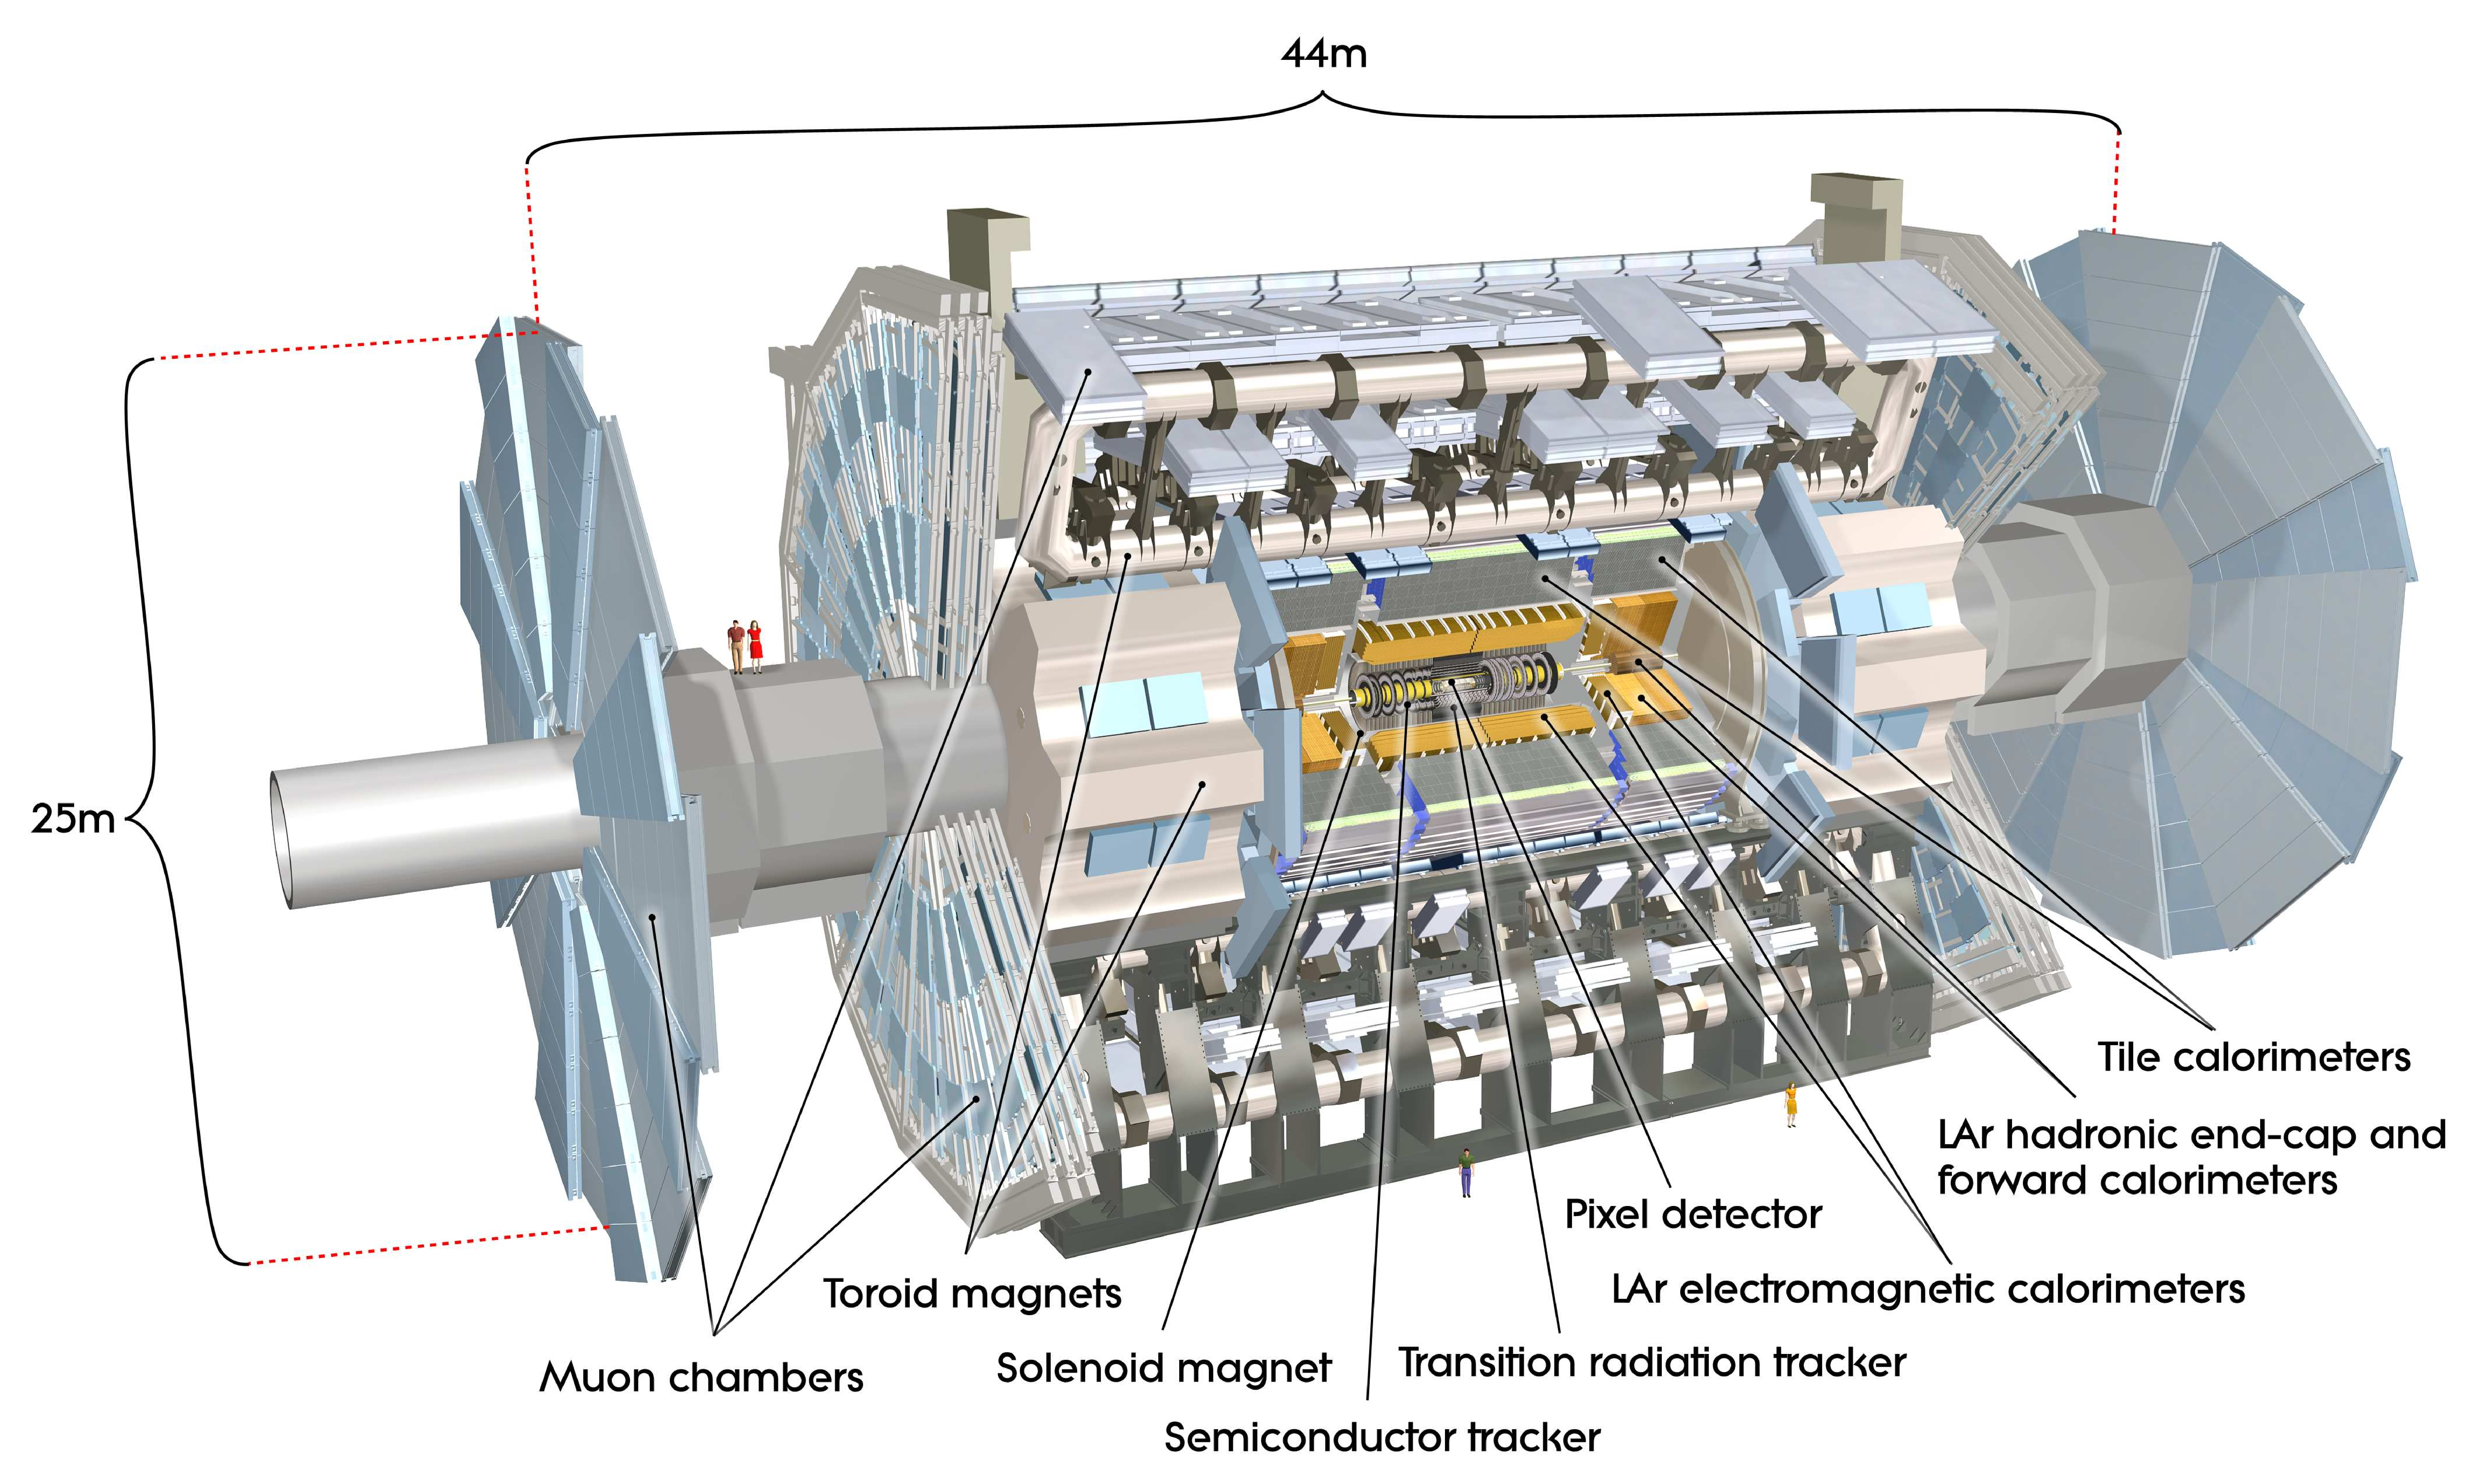
\includegraphics[width=\fullfig]{figures/atlas_overview.pdf}
\caption{A cut-away schematic of the layout of the \ac{ATLAS} detector. Each of the major subsystems is indicated.}
\label{fig:atlas_overview}
\end{figure}

\begin{figure}[hbtp]
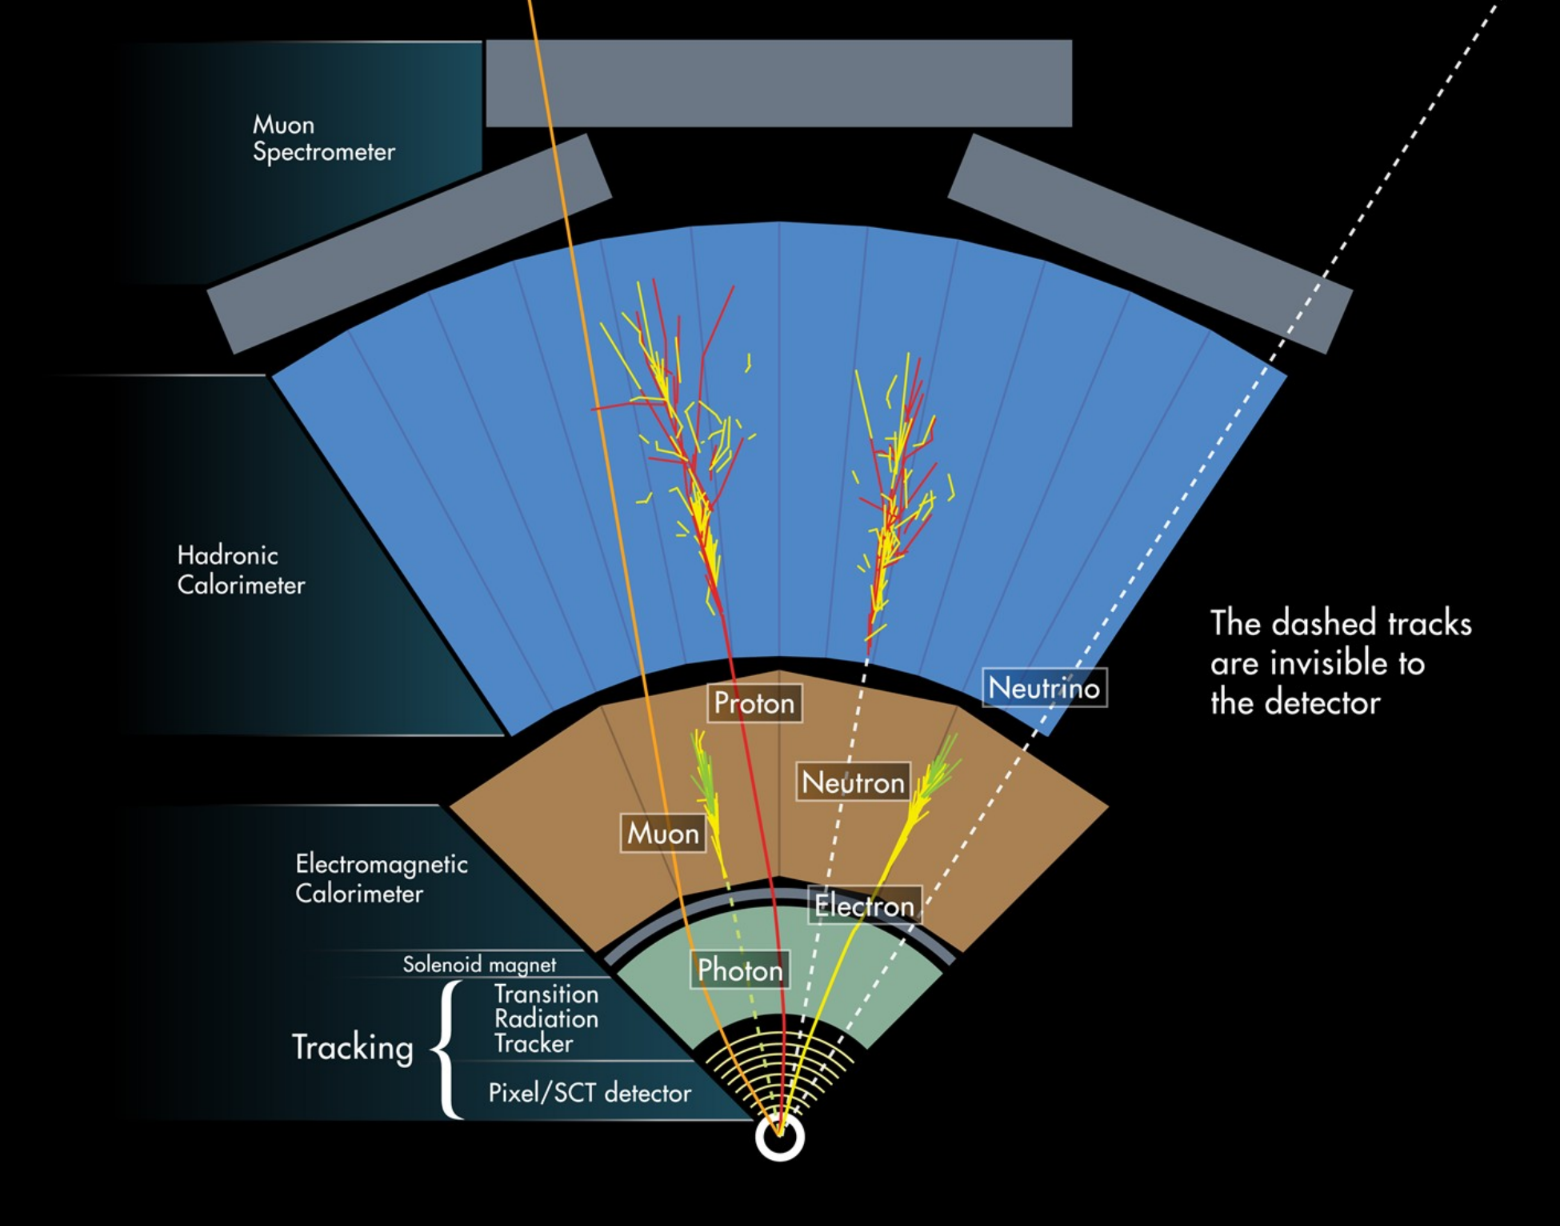
\includegraphics[width=\fullfig]{figures/particle_interactions.png}
\caption{A cross-sectional slice of the \ac{ATLAS} experiment which illustrates how the various \ac{SM} particles interact with the detector systems.}
\label{fig:particle_interactions}
\end{figure}

\begin{table}
\centering
\begin{tabular}{llcc}
  \hline
  Detector Component & Required Resolution & \multicolumn{2}{c}{$|\eta|$ Coverage} \\
                     &                     & Measurement & Trigger \\
  \hline
  Tracking & $\sigma_{\pt}/\pt = 0.05\% \pt + 1\%$ & $2.5$ & - \\
  EM Calorimetry & $\sigma_{E}/E = 10\%/\sqrt{E} + 0.7\%$ & $3.2$ & $2.5$ \\
  Hadronic Calorimetry & & \\
  \quad Barrel and End-Cap & $\sigma_{E}/E = 50\%/\sqrt{E} + 3\%$ & $3.2$ & $3.2$ \\
  \quad Forward & $\sigma_{E}/E = 100\%/\sqrt{E} + 10\%$ & $3.1 - 4.9$ & $3.1 - 4.9$ \\
  Muon Spectrometer & $\sigma_{\pt}/\pt = 10\%$ at $p_T = 1\ \TeV$ & $2.7$ & $2.4$ \\
  \hline
\end{tabular}
\caption{The performance goals for each of the subsystems of the \ac{ATLAS} detector. The $|\eta|$ coverage specifies the range where the subsystem needs to be able to provide measurements with the specified resolution. The resolutions include a \pt or E dependence that is added in quadrature with a \pt/E independent piece.}
\label{tab:performance_goals}
\end{table}

Incorporating these various pieces into a single detector is a significant technical challenge.
The resulting detector has a diameter of 22 m, is 46 m long, and weighs 7,000 tons; it is the largest volume particle detector ever constructed.
The various detector elements need to be constructed and assembled with precisions as low as micrometers.
These systems all need to function well even after exposure to the significant radiation dose from the collisions.
Designing, constructing, and installing the detector took the combined effort of more than 3000 scientists from 38 countries over almost two decades.


\section{Coordinate System}

The coordinate system defined for the \ac{ATLAS} detector is used throughout all of the sections of this thesis.
The choice of coordinate system reflects the cylindrical symmetry of the \ac{ATLAS} detector, and is oriented by the direction of the beamline which defines the $z$-direction.
The positive $z$ side of the detector is commonly referred to as the $A$-side, and the negative $z$ side is referred to as the $C$-side.
The $x-y$ plane is then the plane transverse to the beam direction, with the $x$ direction defined as pointing from the interaction point to the center of the \ac{LHC} ring and the $y$ direction defined as pointing upwards.
The nominal interaction point is the origin of this system.

It is more convenient in practice to use a cylindrical coordinate system.
The angle from the $z$-axis is $\theta$.
The azimuthal angle uses the usual definition, with $\phi$ running around the $z$-axis and $\phi = 0$ corresponding to the $x$-axis.
Many aspects of the detector are independent of the this coordinate to first order.
The remaining direction is typically specified using rapidity or pseudorapidity, where rapidity is defined as

\begin{equation}\label{eq:rapidity}
y = \frac{1}{2} \ln \frac{E + p_z}/{E - p_z}
\end{equation}

\noindent Rapidity is particularly useful to indicate the component along the $z$ direction because differences in rapidity are invariant to boosts along the $z$-direction.
A similar quantity which depends only the $\theta$ is pseudorapidity, 

\begin{equation}\label{eq:pseudorapidity}
\eta = - \ln \tan \frac{\theta}{2}
\end{equation}

\noindent which is the same as rapidity when the particle is massless and in the limit where the energy is much larger than the particle's mass.
It is often useful to refer to differences in solid angle using the pseudorapdity and the azimuthal angle:

\begin{equation}\label{eq:deltar}
\Delta R = \sqrt{\Delta \phi^2 + \Delta \eta^2}
\end{equation}


The pseudorapdity is also invariant to boosts along the $z$-axis for high momentum particles, and is preferable to rapidity because it does not depend on the specific choice of particle.
Pseudorapidity is also preferable to $\theta$ because of the afformentioned boost-invariance and also because particle production is roughly uniform in equal-width intervals of $\eta$ up to about $\eta = 5.0$. 
A particle travelling along the beampipe has $\eta = \inf$ and a particle travelling perpendicular to the beampipe has $\eta = 0$.
The extent of the tracker, $|\eta| < 2.5$, corresponds to approximately $0.05 \pi < \theta [\mathrm{rad}] < 0.95 \pi$ and the extent of the calorimeters, $|\eta| < 4.9$ corresponds to approximately $0.005 \pi < \theta [\mathrm{rad}] < 0.995 \pi$.
Many detector components are broken into multiple subsystems to provide coverage at greater $|\eta|$.
The lower $|\eta|$ region is referred to as the barrel, typically with $|\eta| \lesssim 2$, and the greater $|\eta|$ region is often referred to as the end-cap.

The initial energy and momentum of a proton-proton collision along the $z$ direction is unknown in hadron colliders because different energies and momentums can be carried by the partons.
Along the transverse plane, however, the vector sum of momentum will be zero.
For this reason, many physical quantities are quantified in terms of their projection onto the transverse plan, such as \pt or $E_T$.
In addition, \pt alone determines the amount of curvature in the magnetic field, and can be measured independently by measuring the curvature of a particle's propagation.


\section{Magnetic Field}

The magnet system used in \ac{ATLAS} is designed to provide a substantial magnetic field in the two regions where the trajectory of particles is measured, the inner detector and the muon spectrometer.
The magnetic field provides a curvature to the trajectory of charged particles and allows the precision tracking measurements to make high resolutions measurements of \pt.
To provide a magnetic field in these regions, \ac{ATLAS} uses a hybrid system with four separate, superconducting magnets.
A single solenoid provides a 2 T axial magnetic field for the inner detector, while a barrel toroid and two end-cap toroids produce a magnetic field of 0.5 and 1 T, respectively, for the muon detectors.
This geometry is illustrated in Figure~\ref{fig:magnets_overview}.

\begin{figure}[hbtp]
\centering
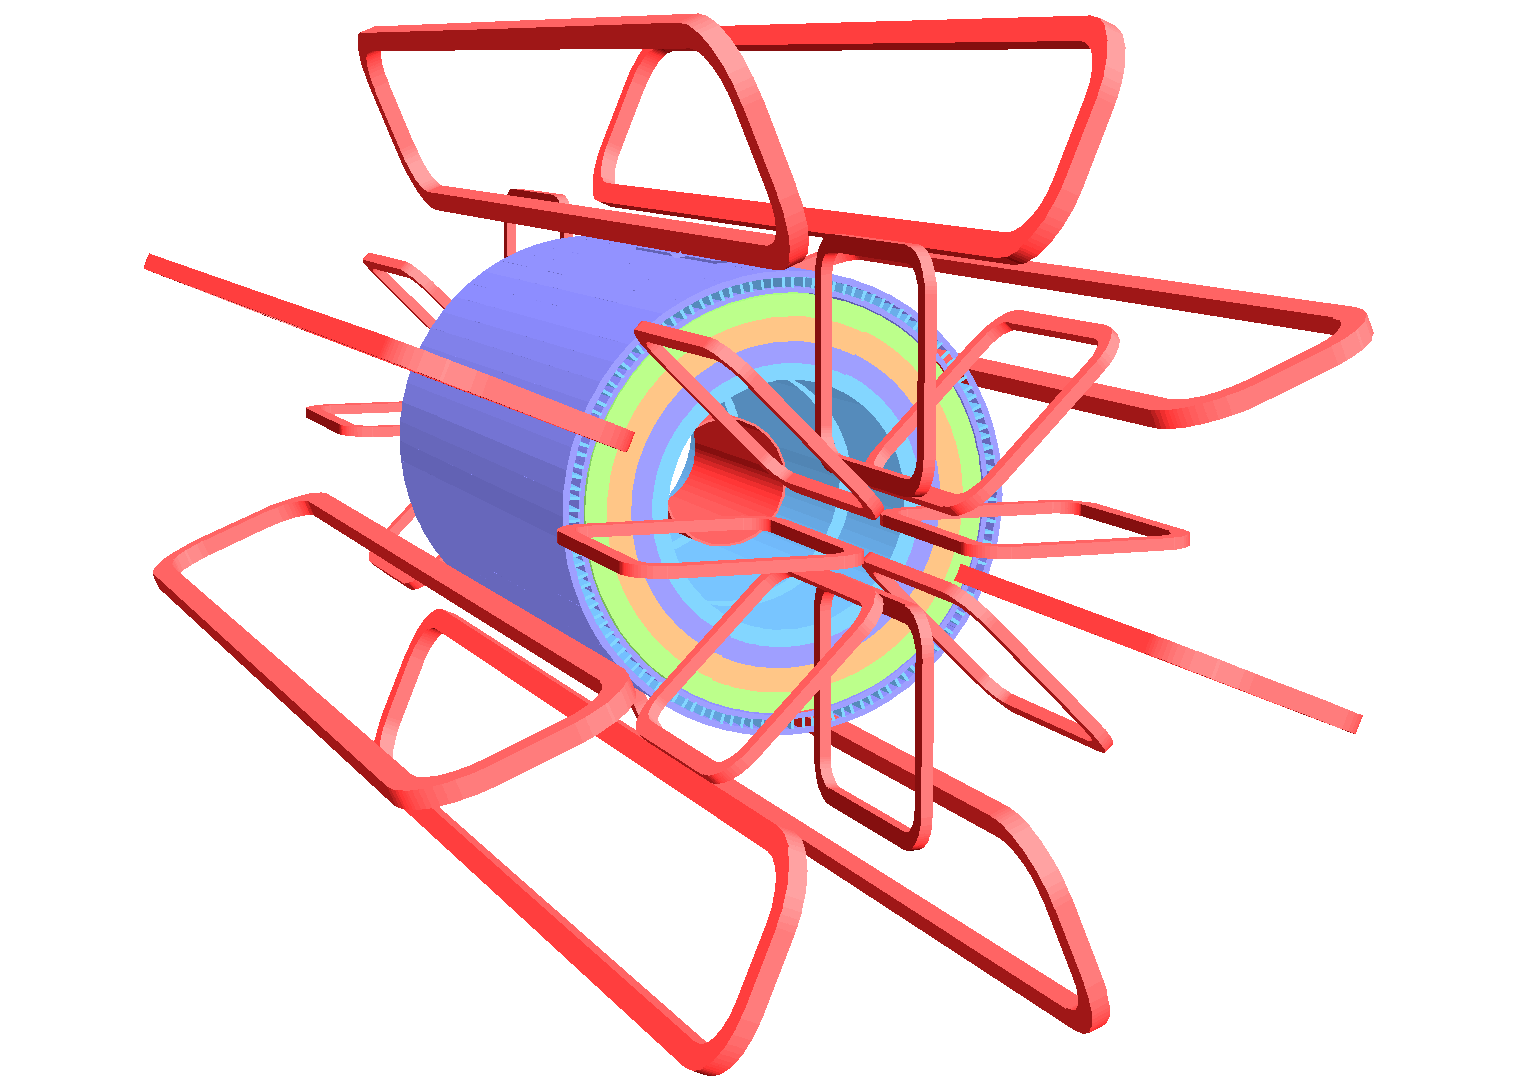
\includegraphics[width=\fullfig]{figures/magnets_overview.pdf}
\caption{The layout of the four superconducting magnets in the \ac{ATLAS} detector.}
\label{fig:magnets_overview}
\end{figure}

The central solenoid uses a single-layer coil with a current of 7.730 kA to generate the 2 T axial field at the center of the magnet. 
The single-layer coil design enables a minimal amount of material to be used in the solenoid's construction, which is important because the solenoid is placed between the inner detector and the calorimeters.
At normal incidence the magnet has only 0.66 radiation lengths worth of material, where one radiation length is the mean distance over which a high-energy electron loses all but $1/e$ of its energy through material interactions~\cite{pdg}.
The coil is made of a high-strength aluminum stabilized NbTi superconductor which was optimized to achieve a high field with minimal thickness.
The axial magnetic field produced by the solenoid bends charged particles in the $\phi$ direction.

The barrel toroid consists of eight coils which generate a 0.5 T magnetic field in the cylindrical region around the calorimeters with an approximately 20 kA current.
The coils are separated only by air to reduce the scattering of muons as they propogate through the region.
The coils are made of an aluminum stabilized NbTiCu superconductor and each is separately housed in a vacuum and cold chamber.
This magnetic configuration produces a field in the $\phi$ and so curves muons traversing the volume primarily in the $\eta$ direction.

The end-cap toroids follow a similar design to the barrel toroid, with eight separate NbTiCu coils, but in this case all eight are housed within a single cold mass.
This extra structure is necessary to withstand the Lorentz forces exerted by the magnets. 
These magnets are rotated 22.5\% relative to the barrel toroid to provide a uniform field in the transition between the two systems. 
The end-cap toroids also produce a field in the $\phi$ direction and curve muons primarily in the $\eta$ direction.

The major parameters of the three magnet systems are summarized in Table~\ref{tab:magnet_parameters}.

\begin{table}
\centering
\begin{tabular}{lcccc}
\hline
Parameter & Unit & Solenoid & Barrel Toroid & End-Cap Toroids \\
\hline
Inner Diamater & m & 2.4 & 9.4 & 1.7 \\
Outer Diamater & m & 2.6 & 20.1 & 10.7 \\
Axial Length & m & 5.3 & 25.3 & 5.0 \\
Weight & tons & 5.7 & 830 & 239 \\
Conductor Size & mm\tsup{2} & 30$\times$4.25 & 57$\times$12 & 41$\times$4.25 \\
Peak Field & T & 2.6 & 3.9 & 4.1\\
Heat Load & W & 130 & 990 & 330 \\
Current & kA & 7.7 & 20.5 & 20.0 \\
Stored Energy & MJ & 38 & 1080 & 206 \\
\hline
\end{tabular}
\end{table}


% ----------------------------------------

\section{Inner Detector}



\begin{figure}[hbtp]
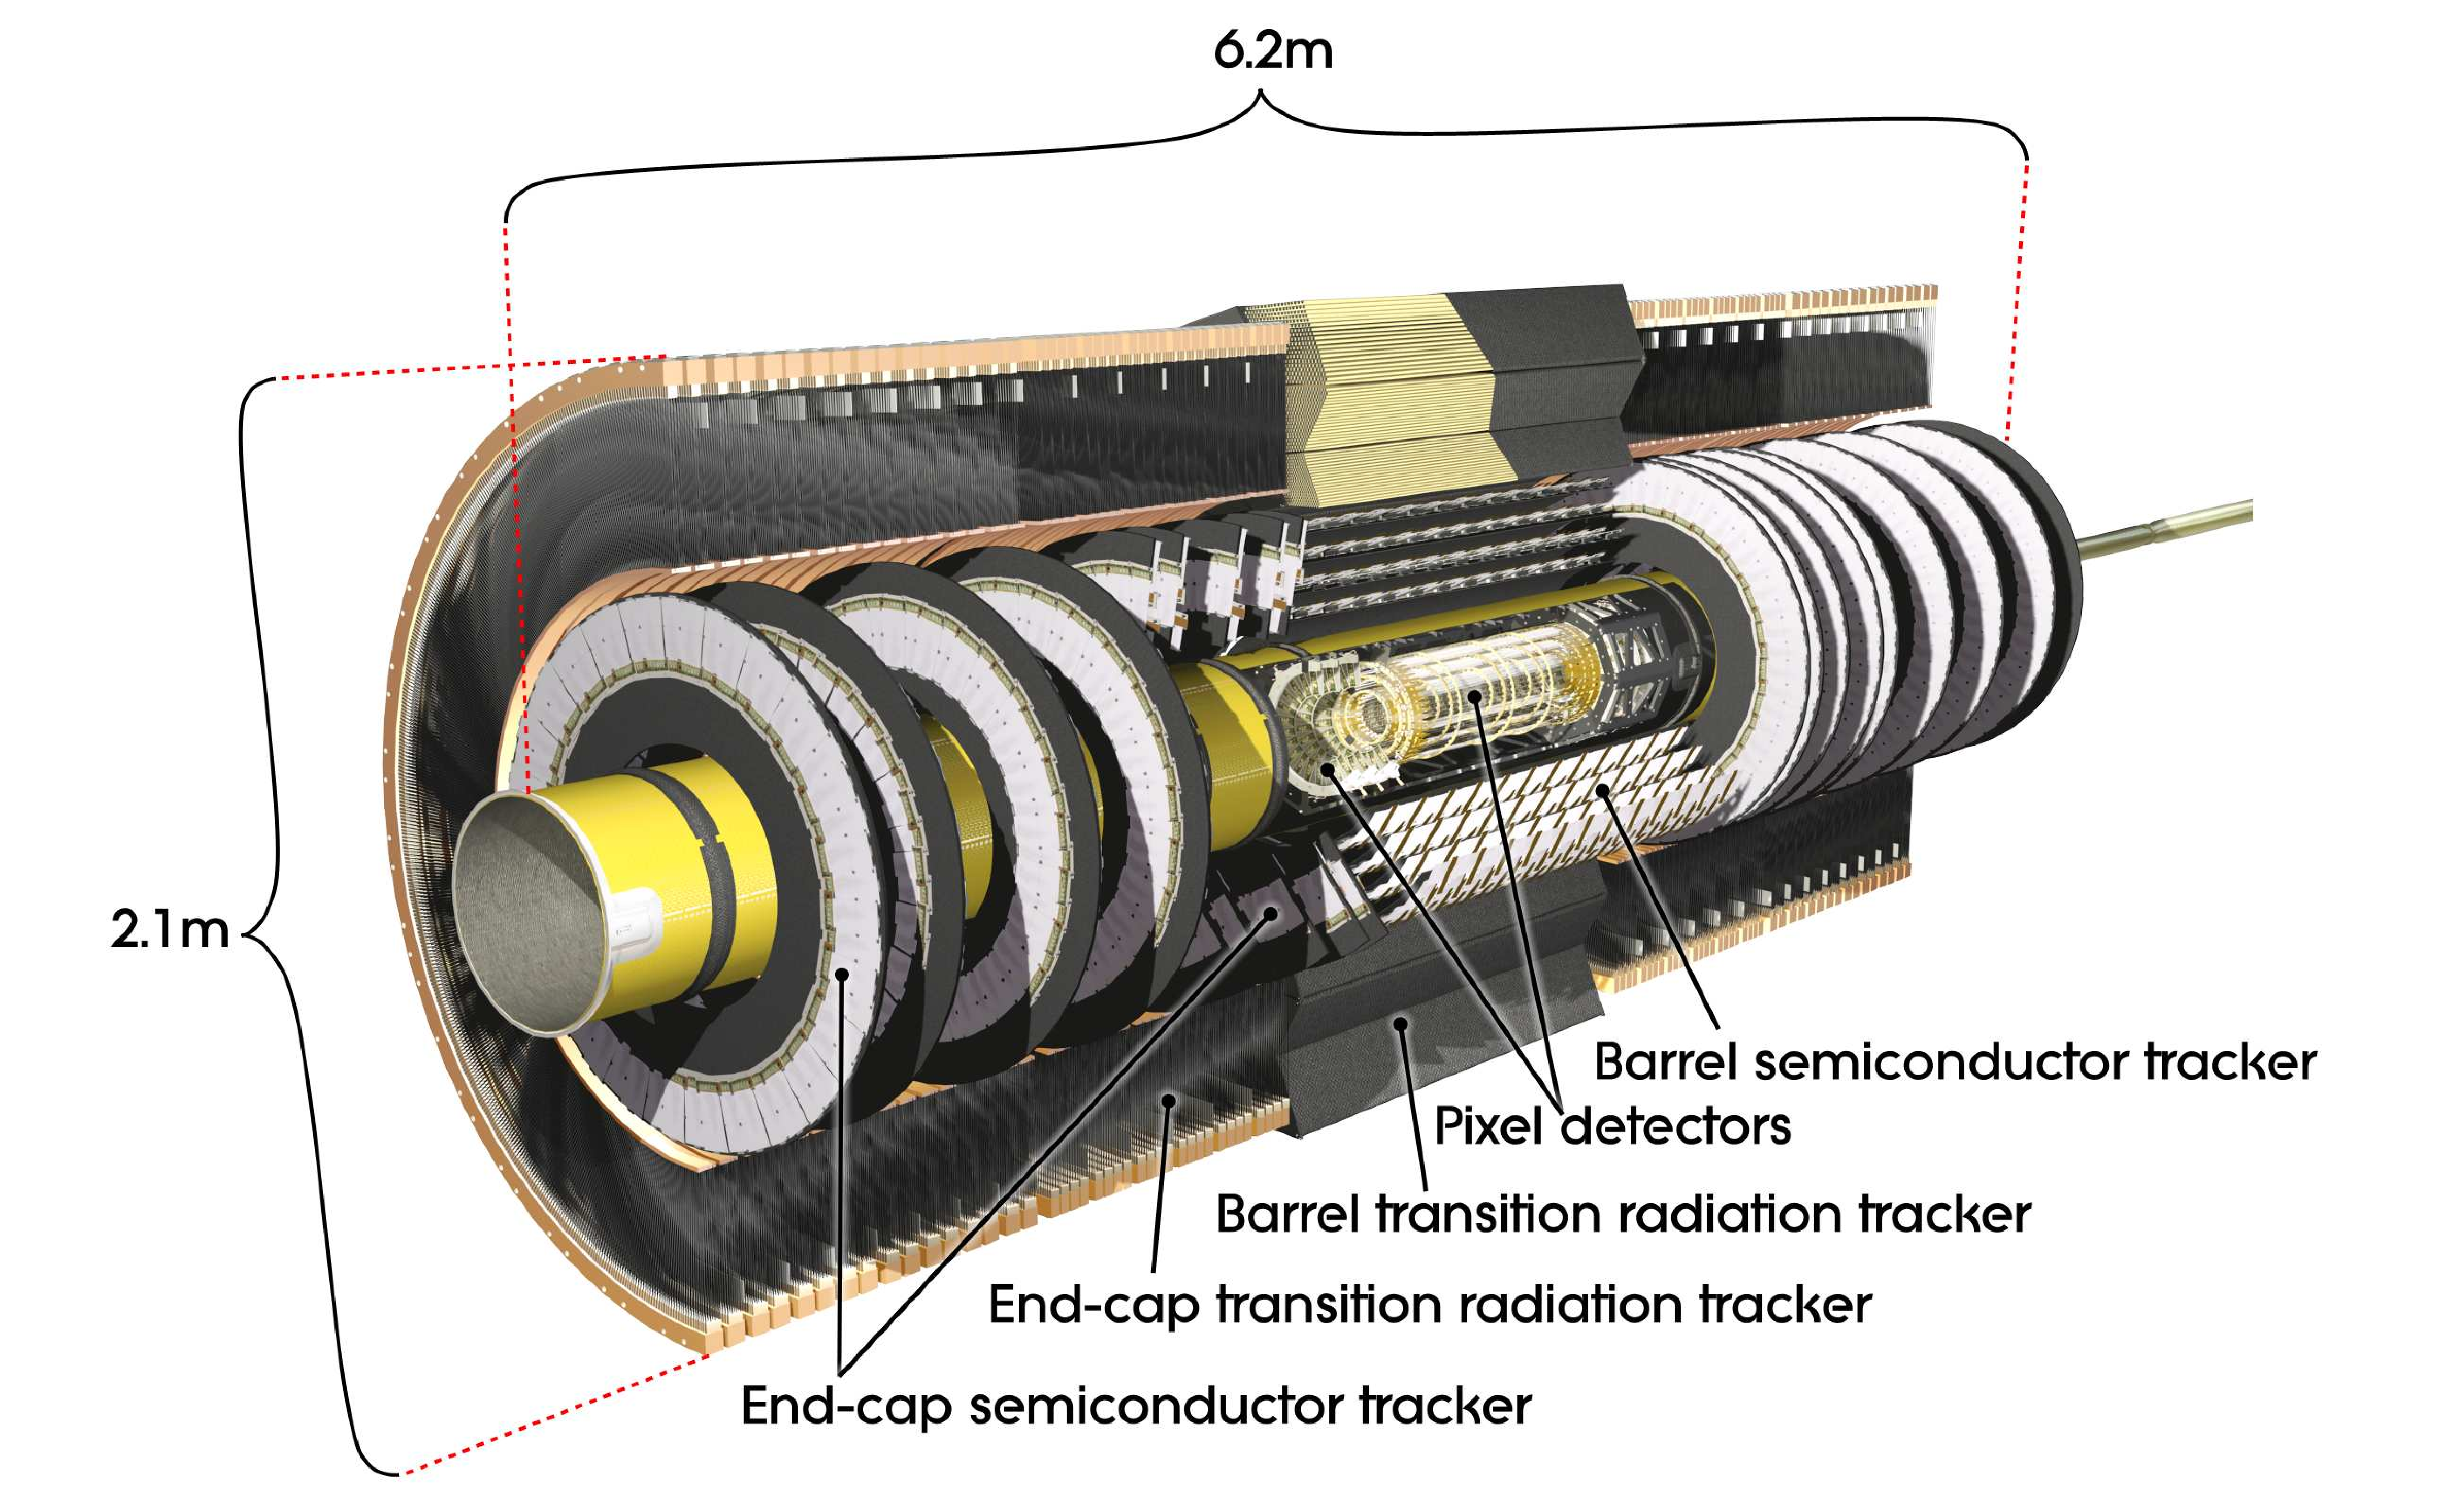
\includegraphics[width=\fullfig]{figures/id_overview.pdf}
\caption{}
\label{fig:id_overview}
\end{figure}

\begin{figure}[hbtp]
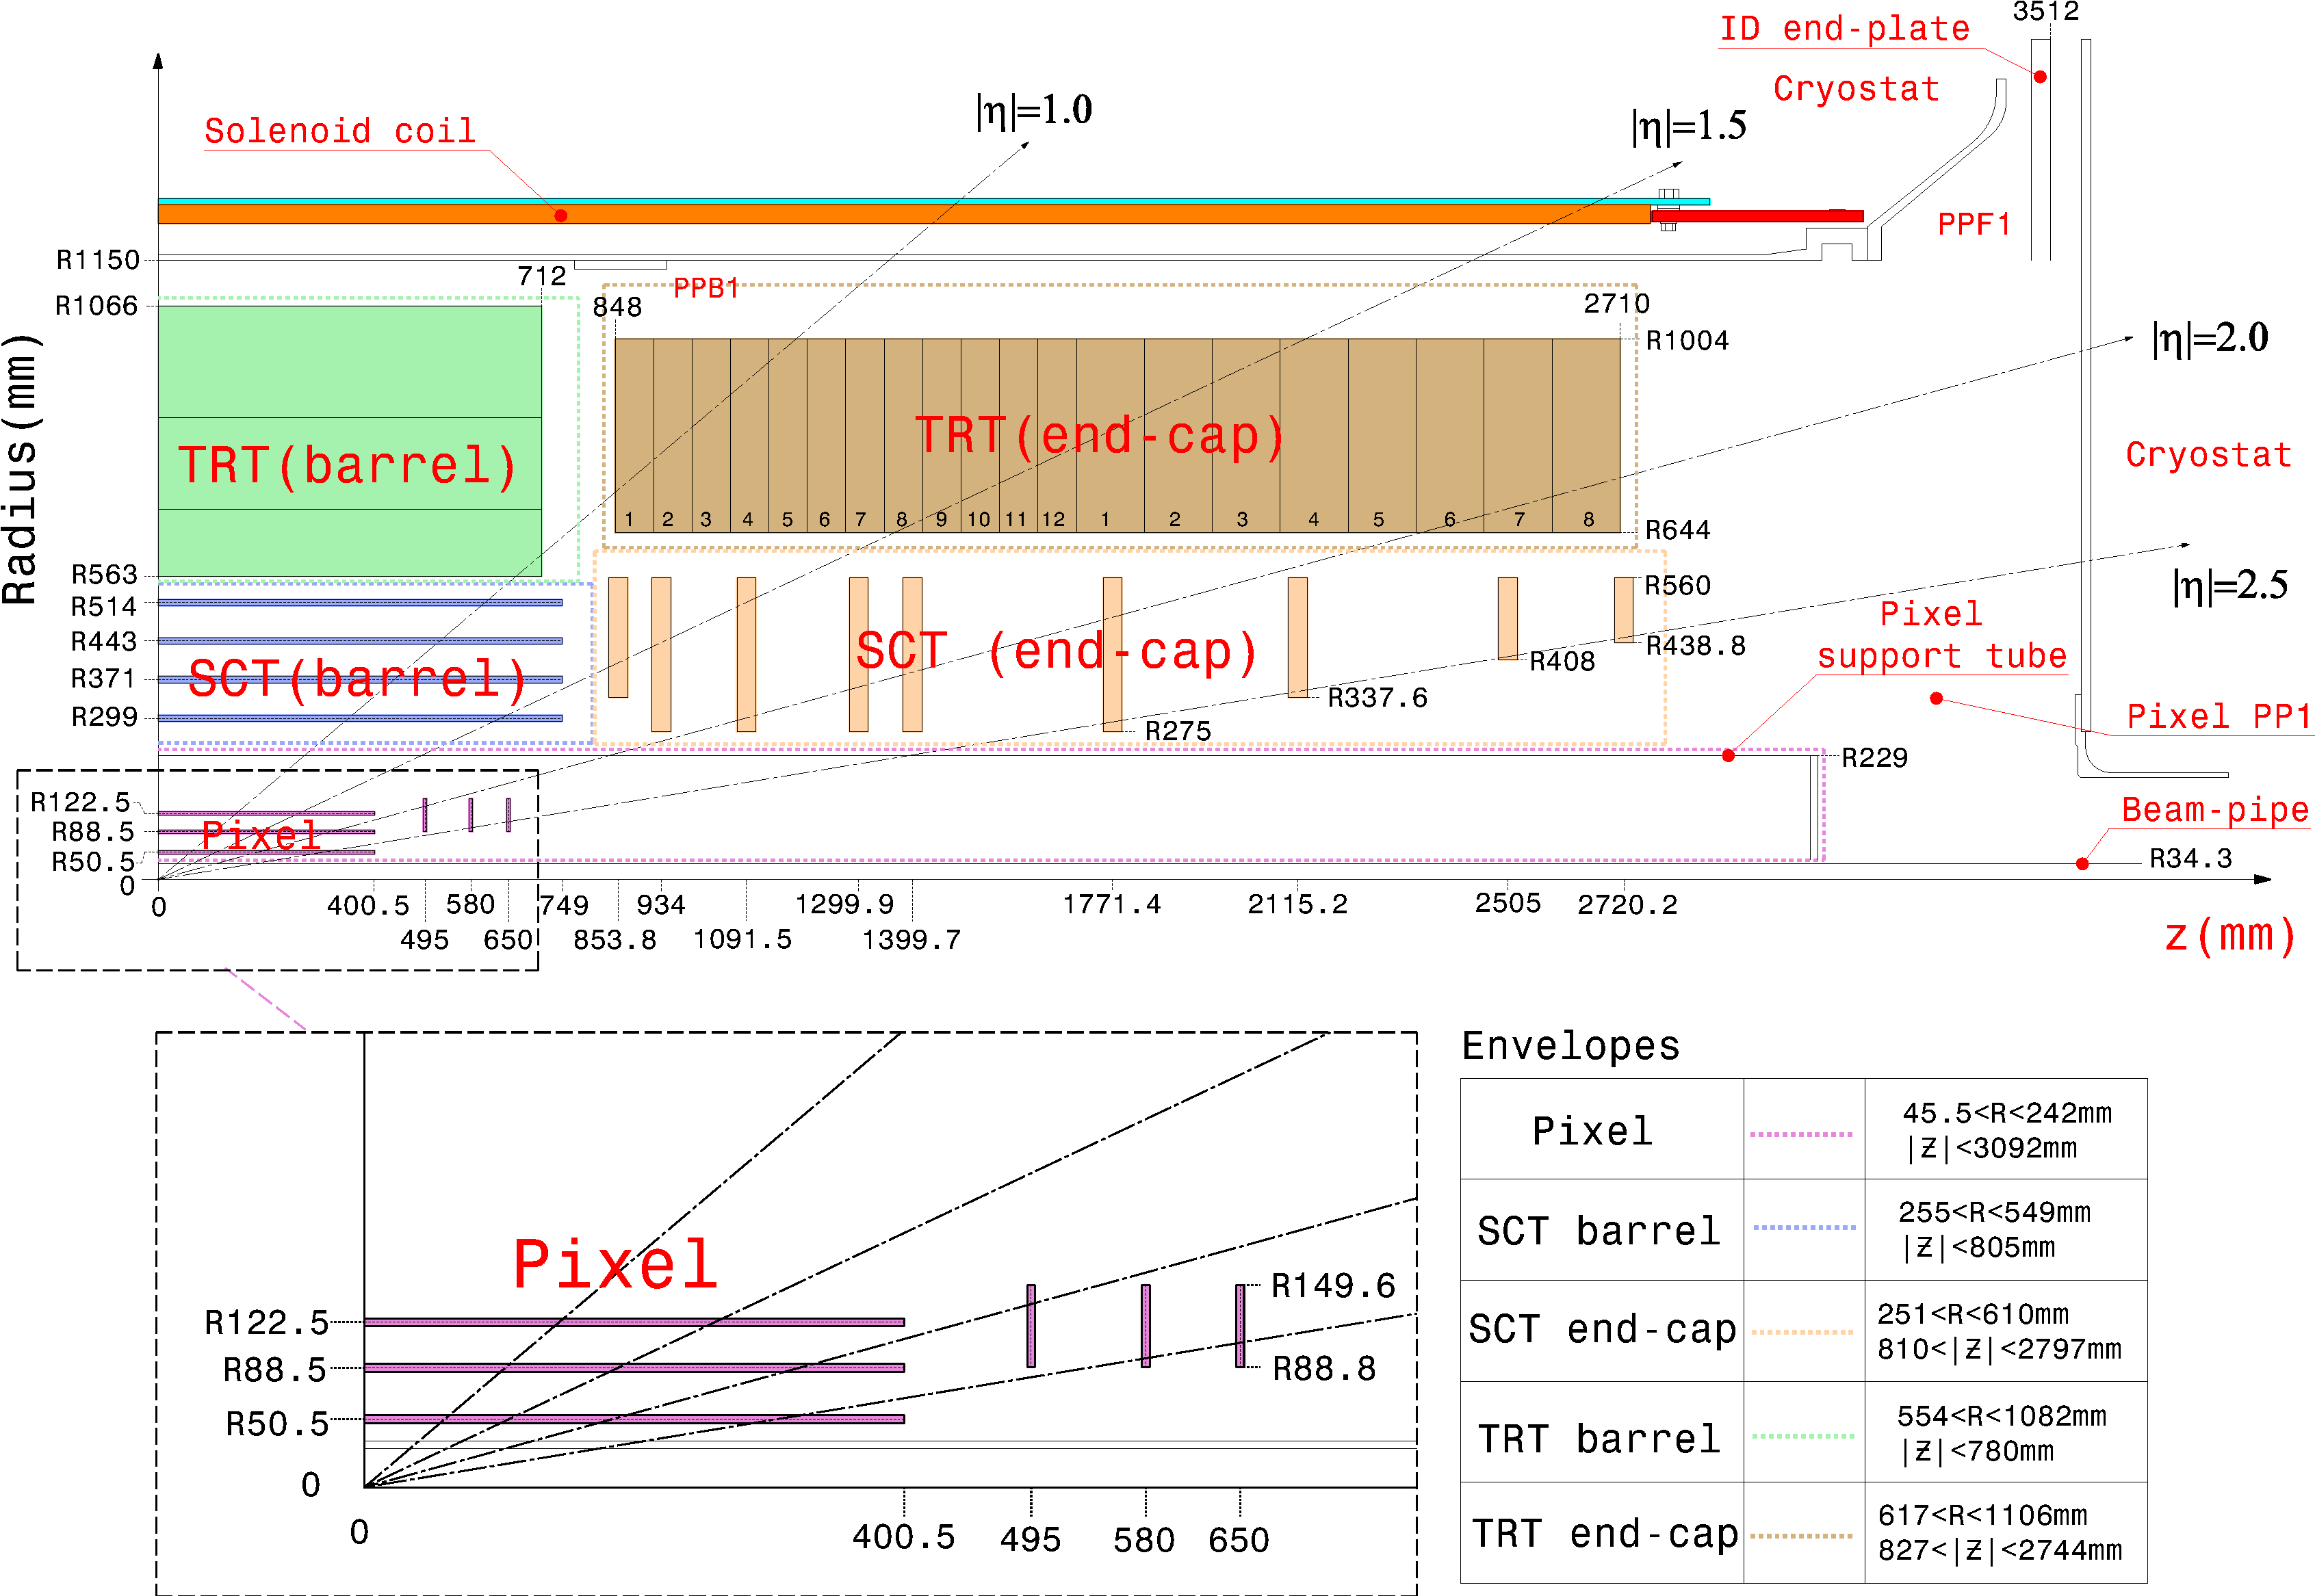
\includegraphics[width=\fullfig]{figures/id_detail_schematic.pdf}
\caption{}
\label{fig:id_detail_schematic}
\end{figure}


\begin{figure}[hbtp]
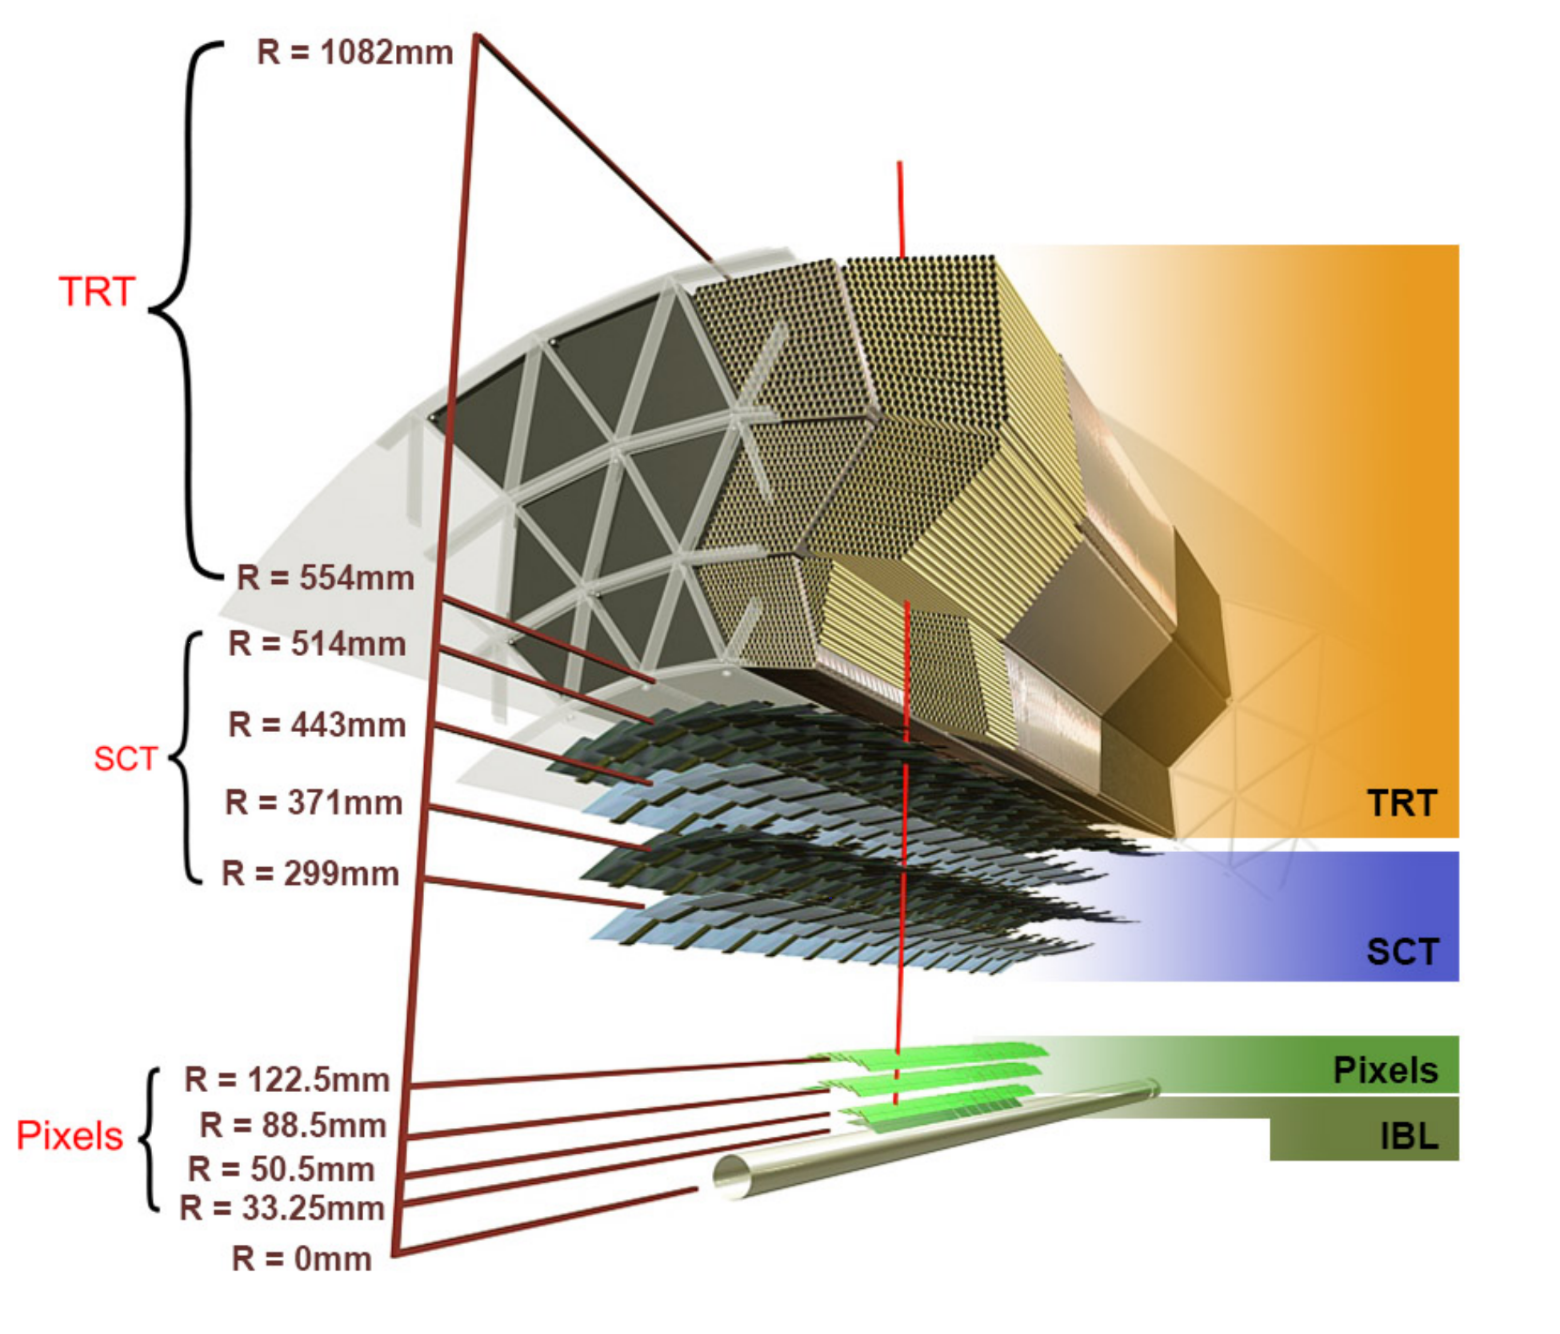
\includegraphics[width=\fullfig]{figures/id_slice.png}
\caption{}
\label{fig:id_slice}
\end{figure}


\begin{figure}[hbtp]
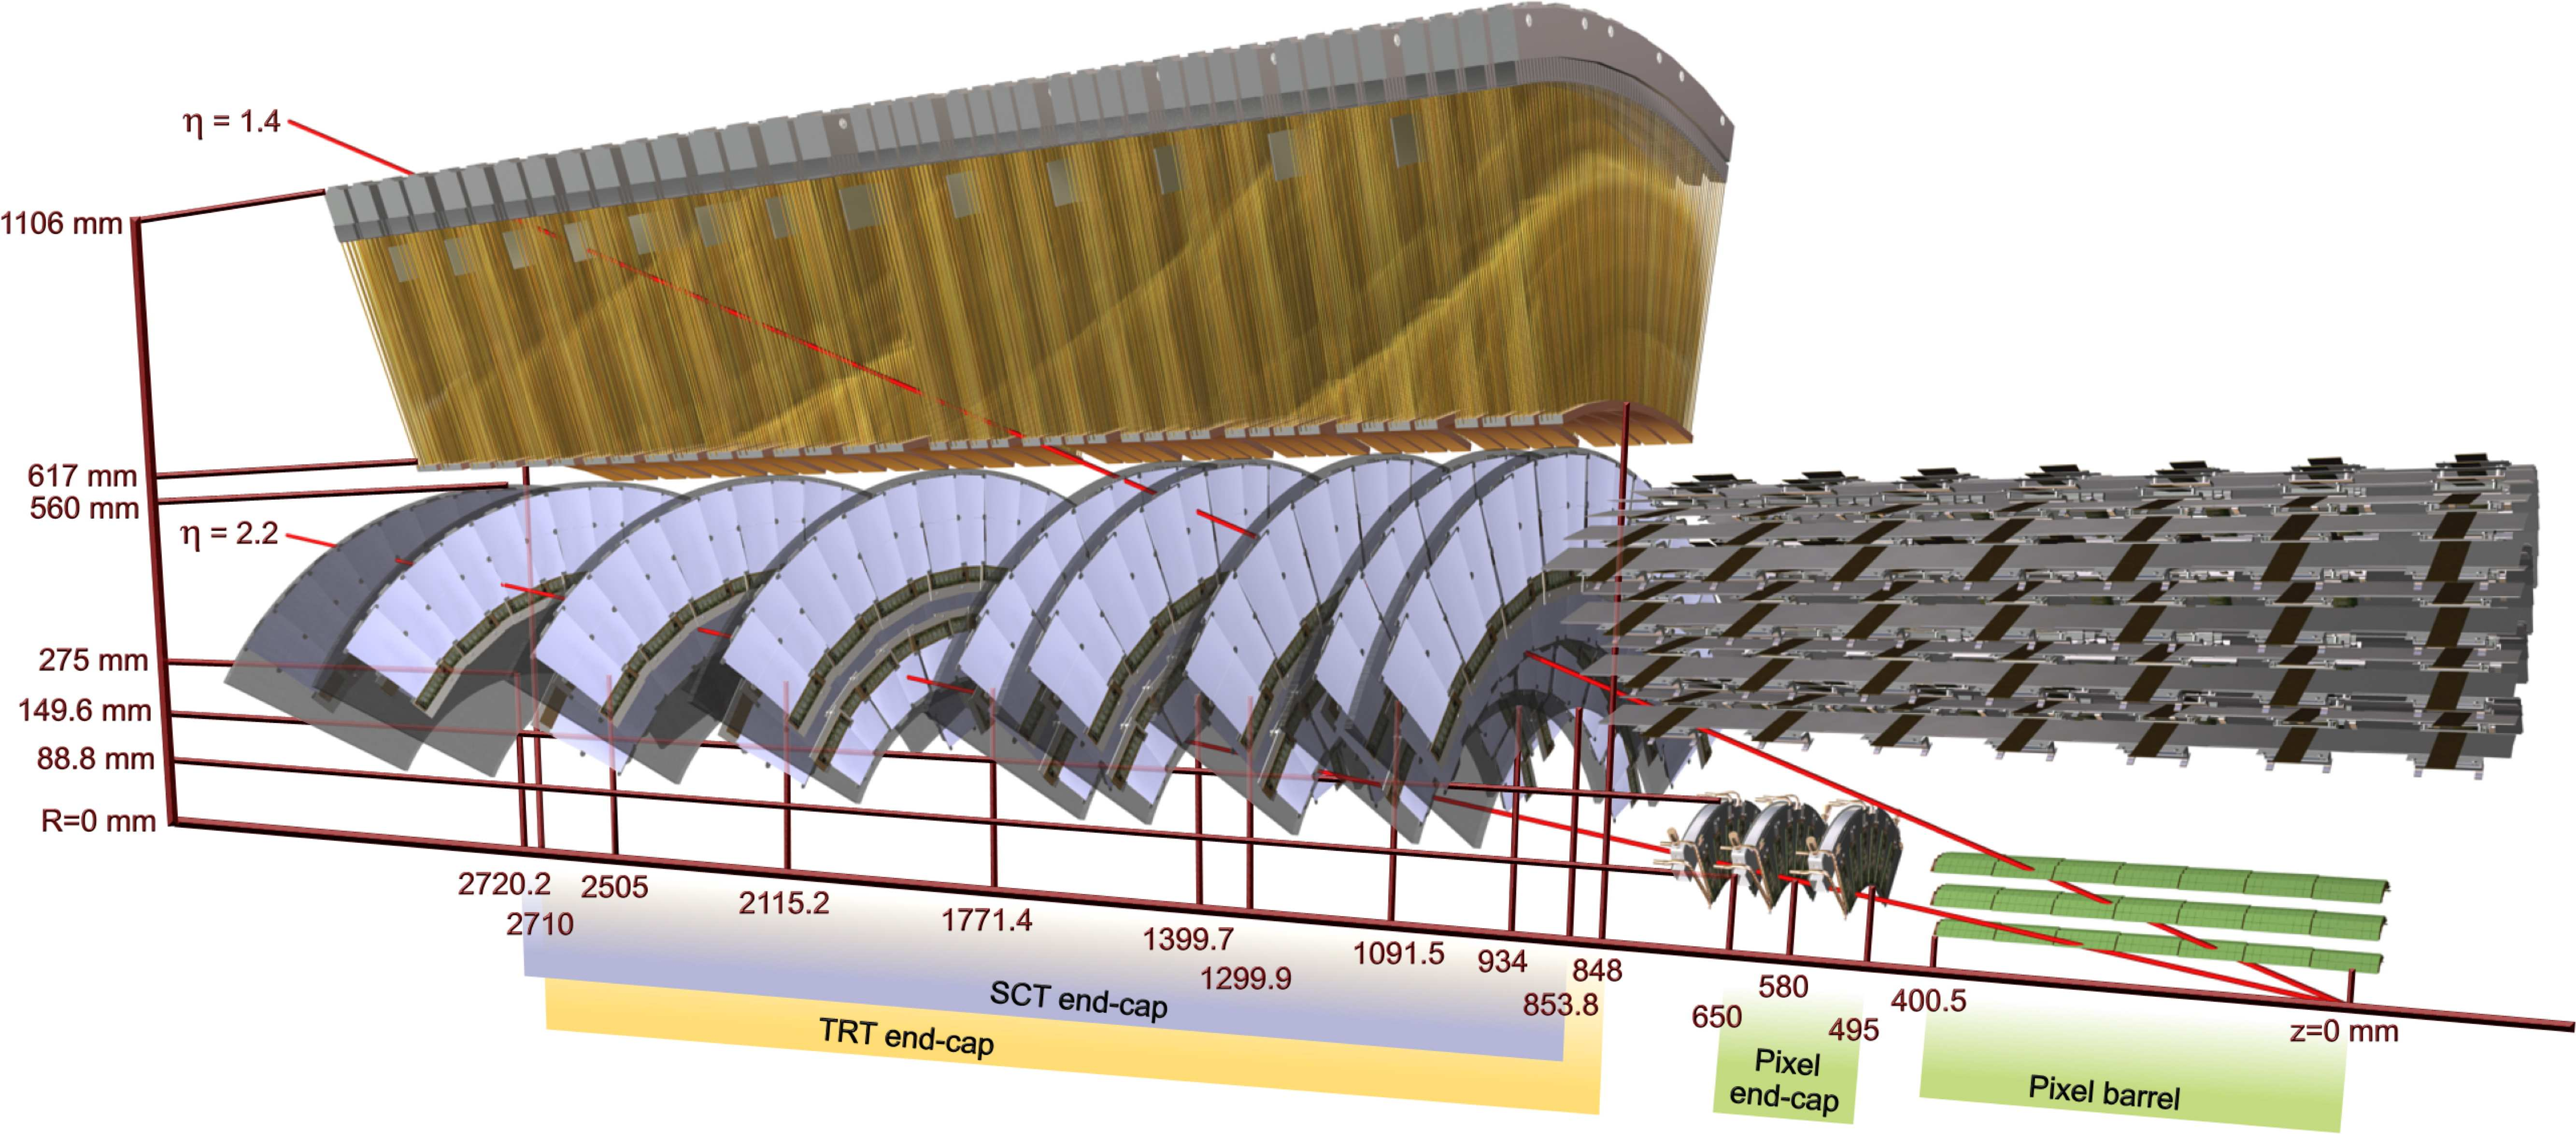
\includegraphics[width=\fullfig]{figures/id_slice_long.pdf}
\caption{}
\label{fig:id_slice_long}
\end{figure}


\subsection{Pixel Detector}
\label{sec:pixel}

\begin{figure}[hbtp]
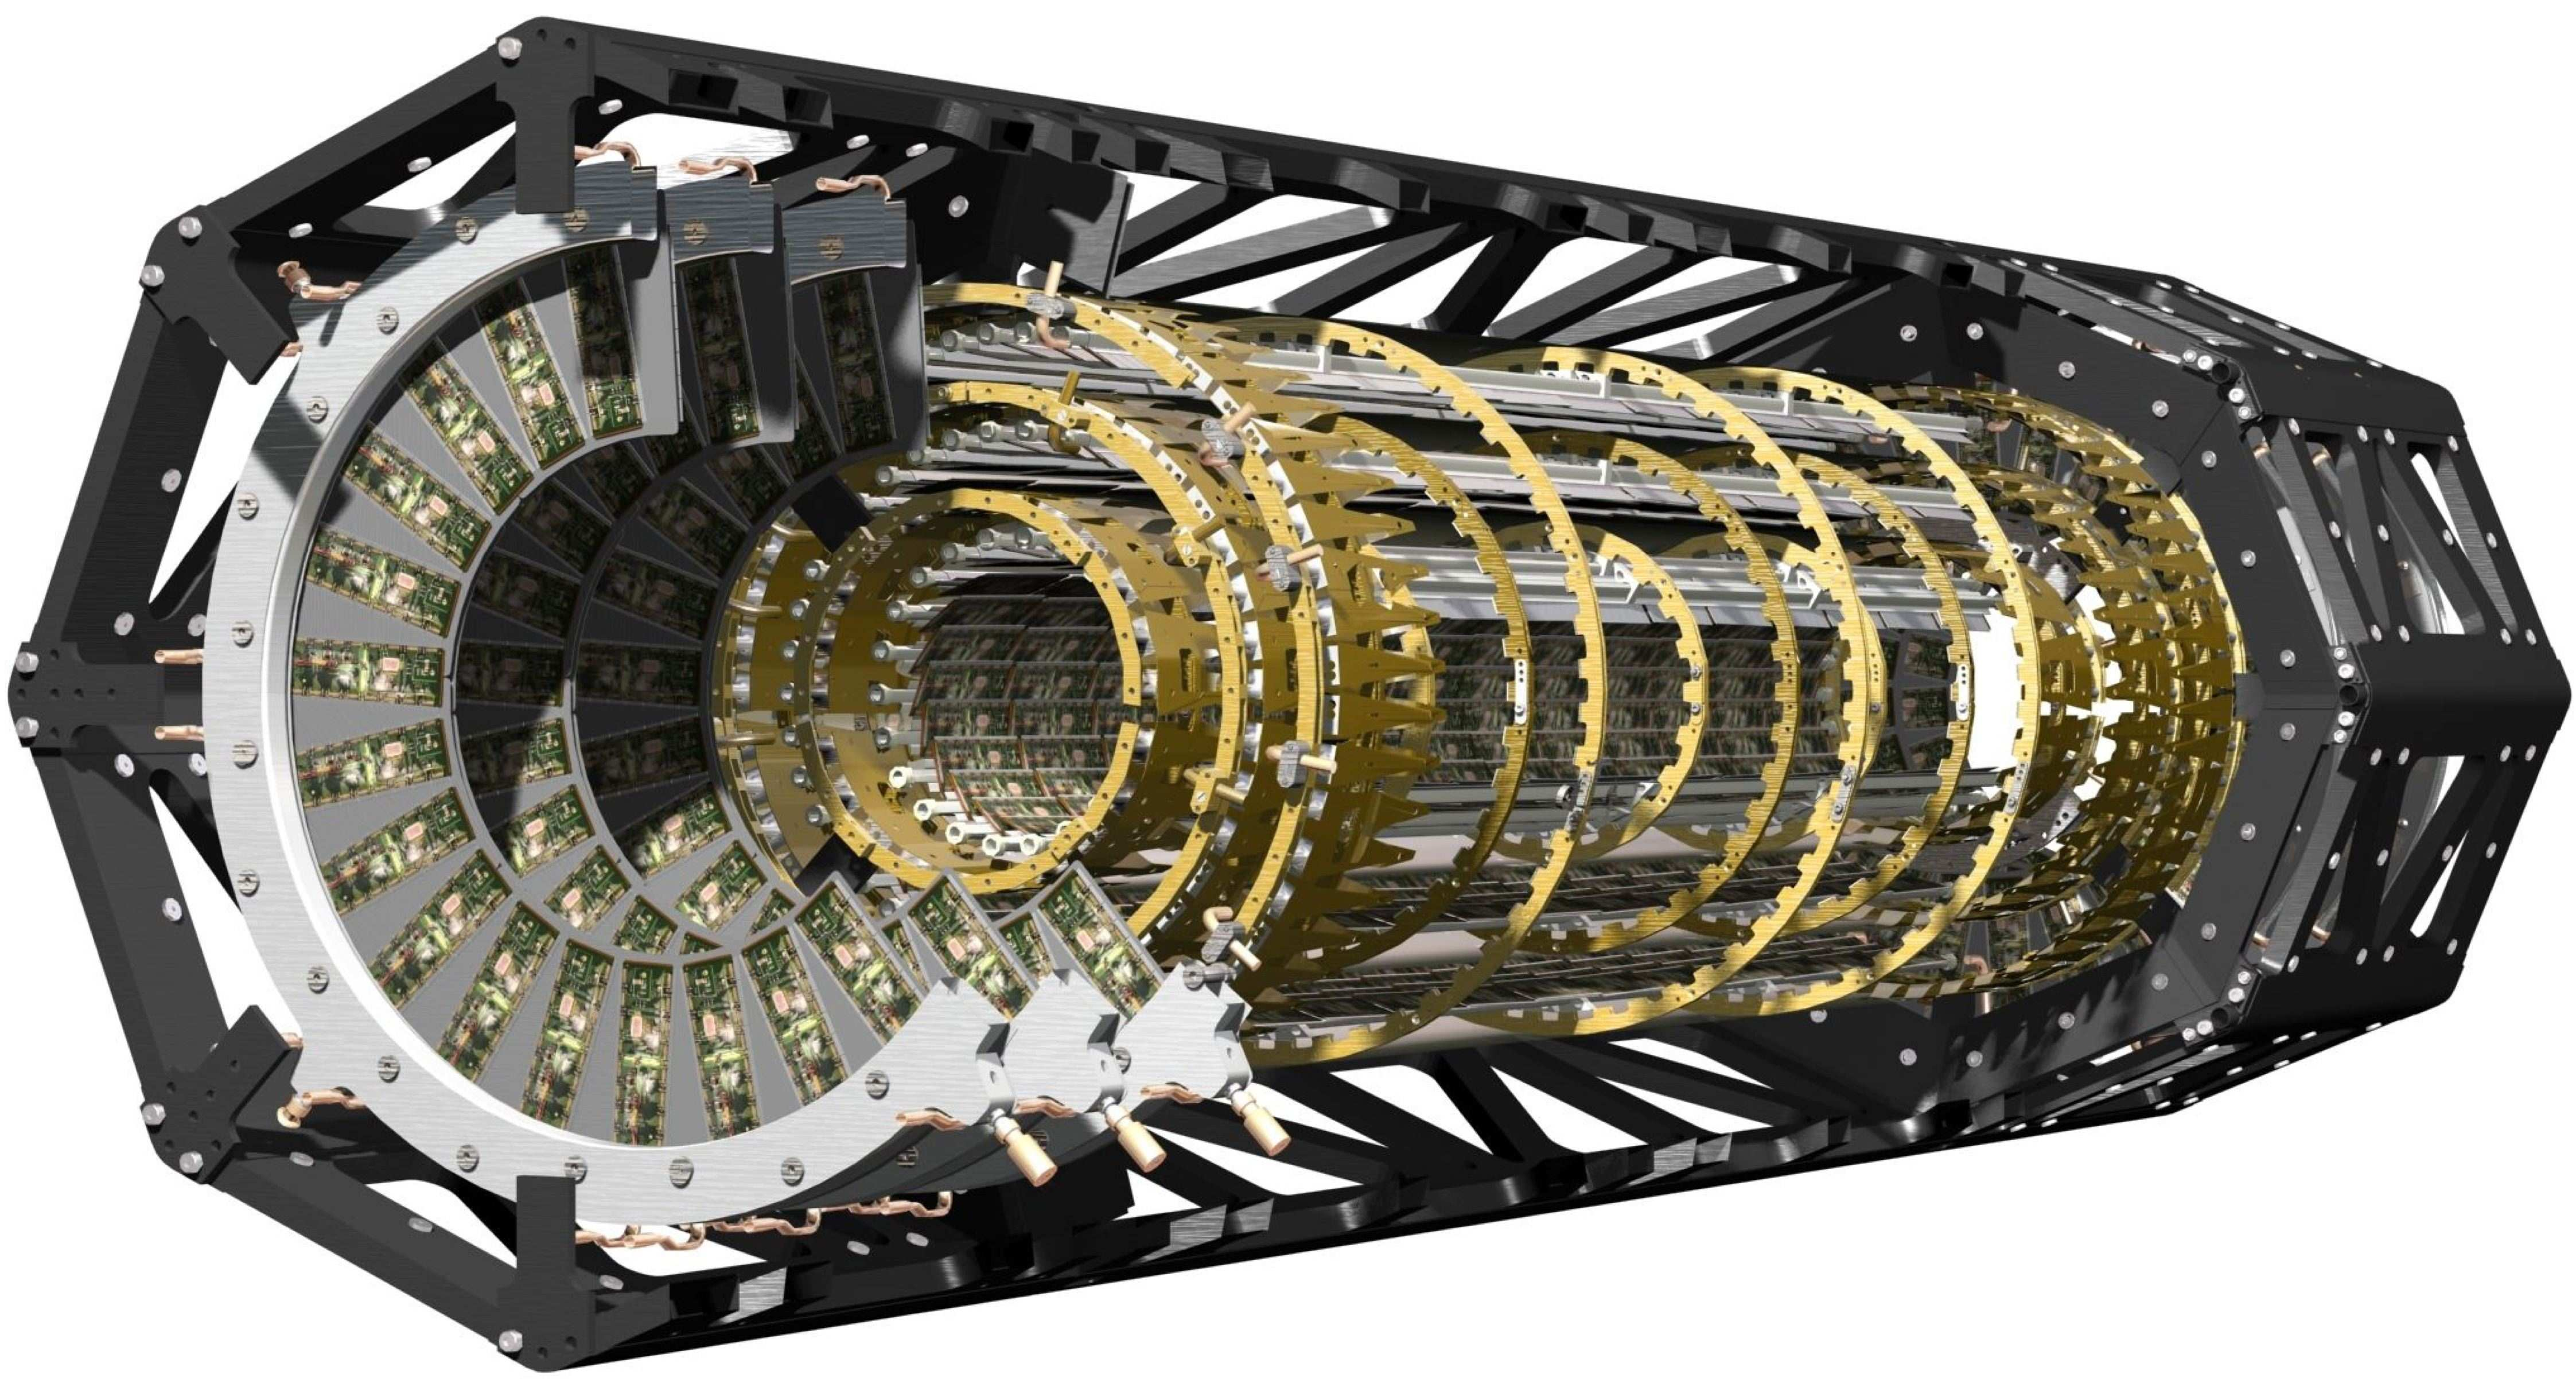
\includegraphics[width=\fullfig]{figures/pixel_overview.pdf}
\caption{}
\label{fig:pixel_overview}
\end{figure}

\begin{figure}[hbtp]
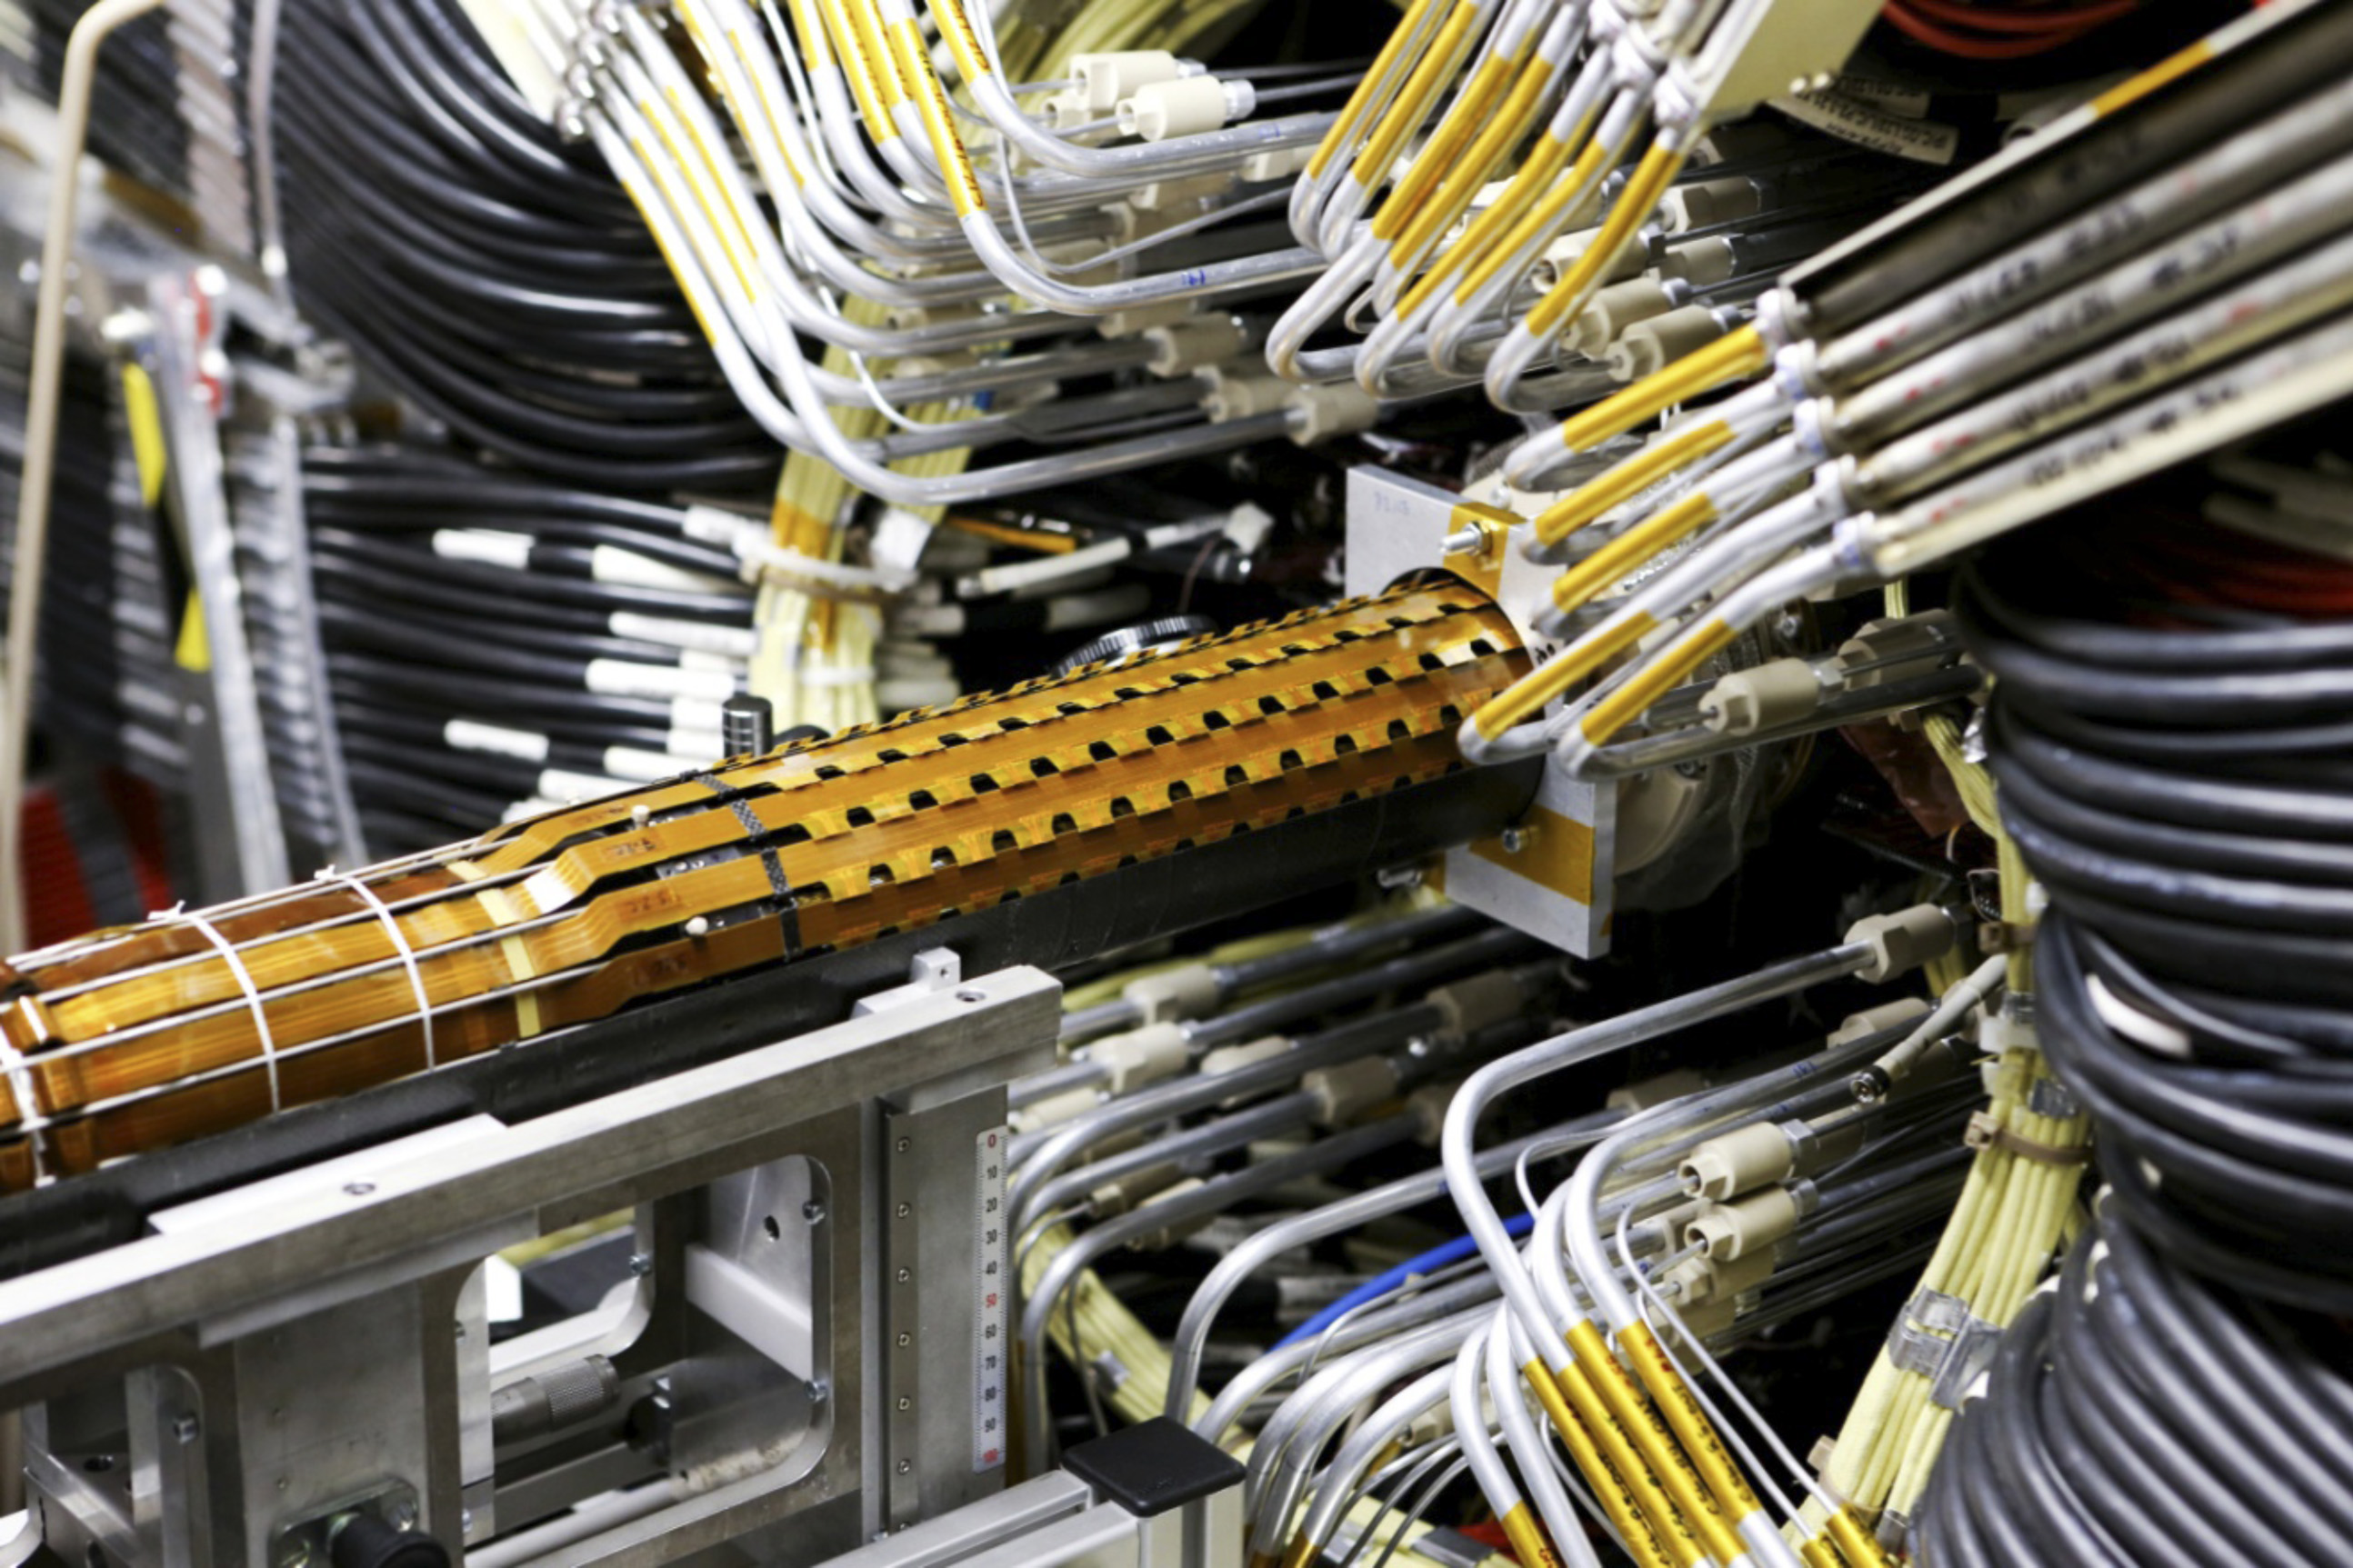
\includegraphics[width=\fullfig]{figures/ibl_insertion.jpg}
\caption{}
\label{fig:ibl_insertion}
\end{figure}


\subsection{Semiconductor Tracker}

\subsection{Transition Radiation Tracker}

% ----------------------------------------

\section{Calorimetry}

\begin{figure}[hbtp]
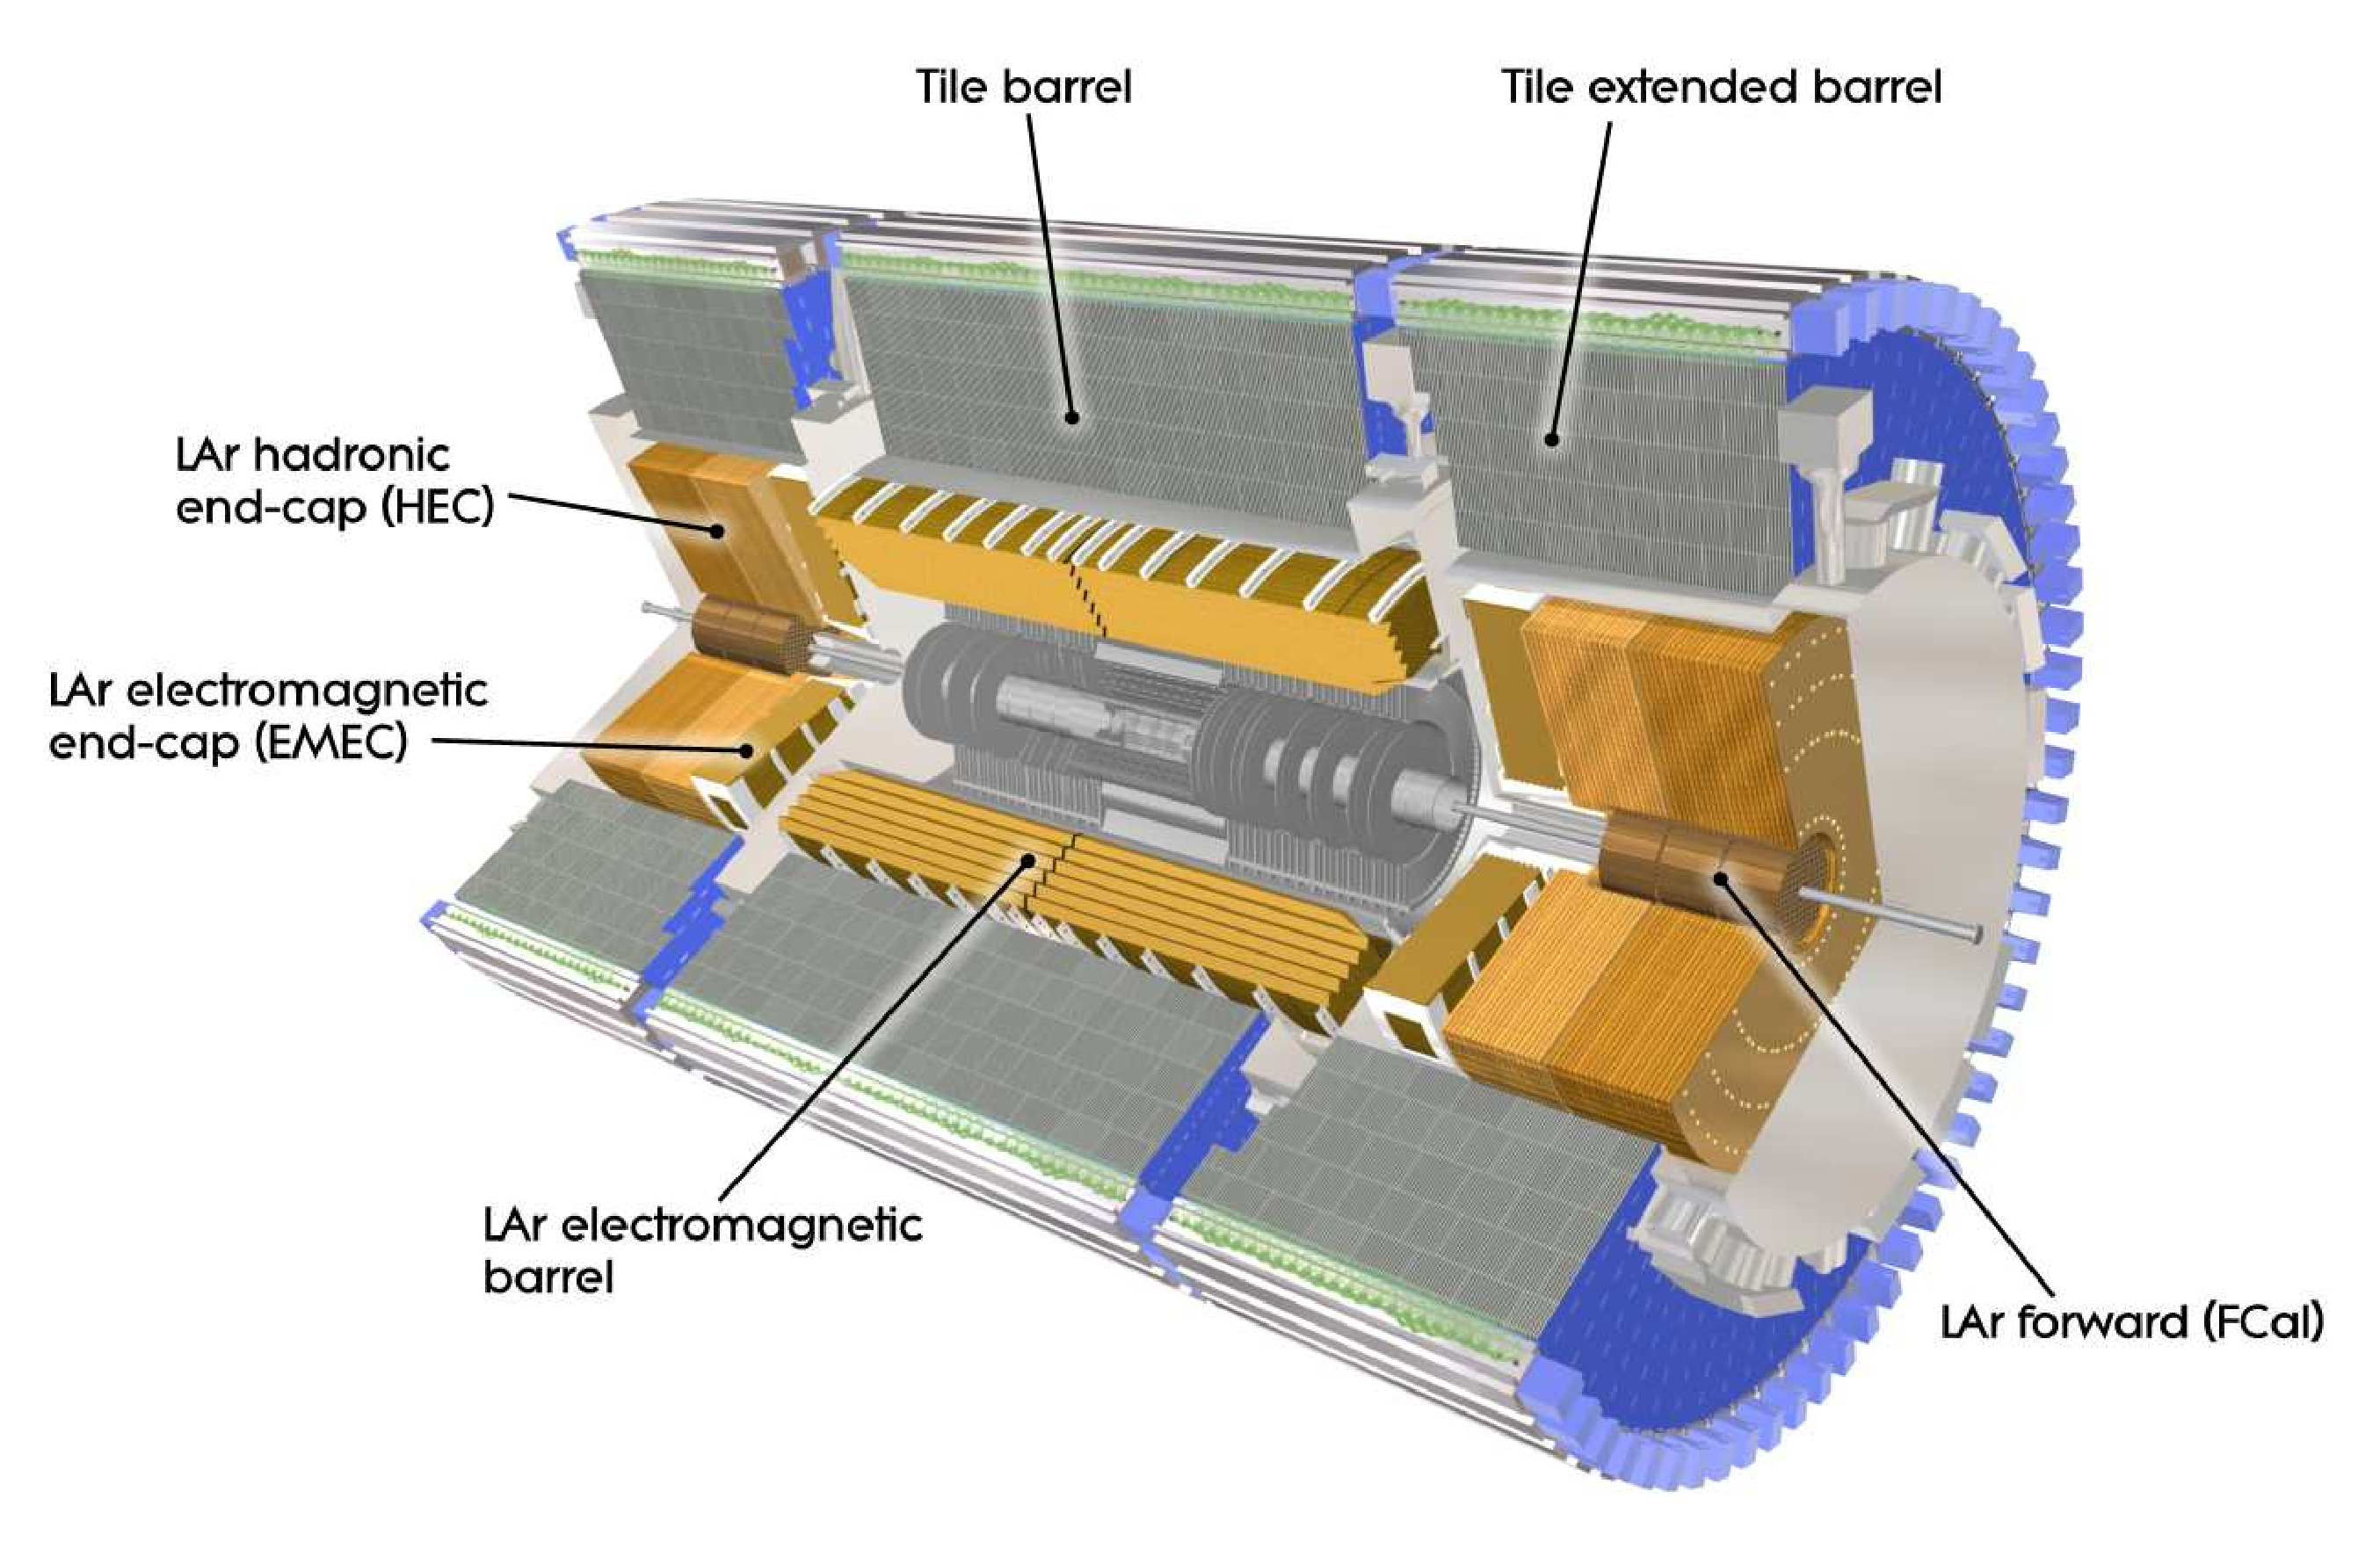
\includegraphics[width=\fullfig]{figures/calo_overview.pdf}
\caption{}
\label{fig:calo_overview}
\end{figure}


\begin{figure}[hbtp]
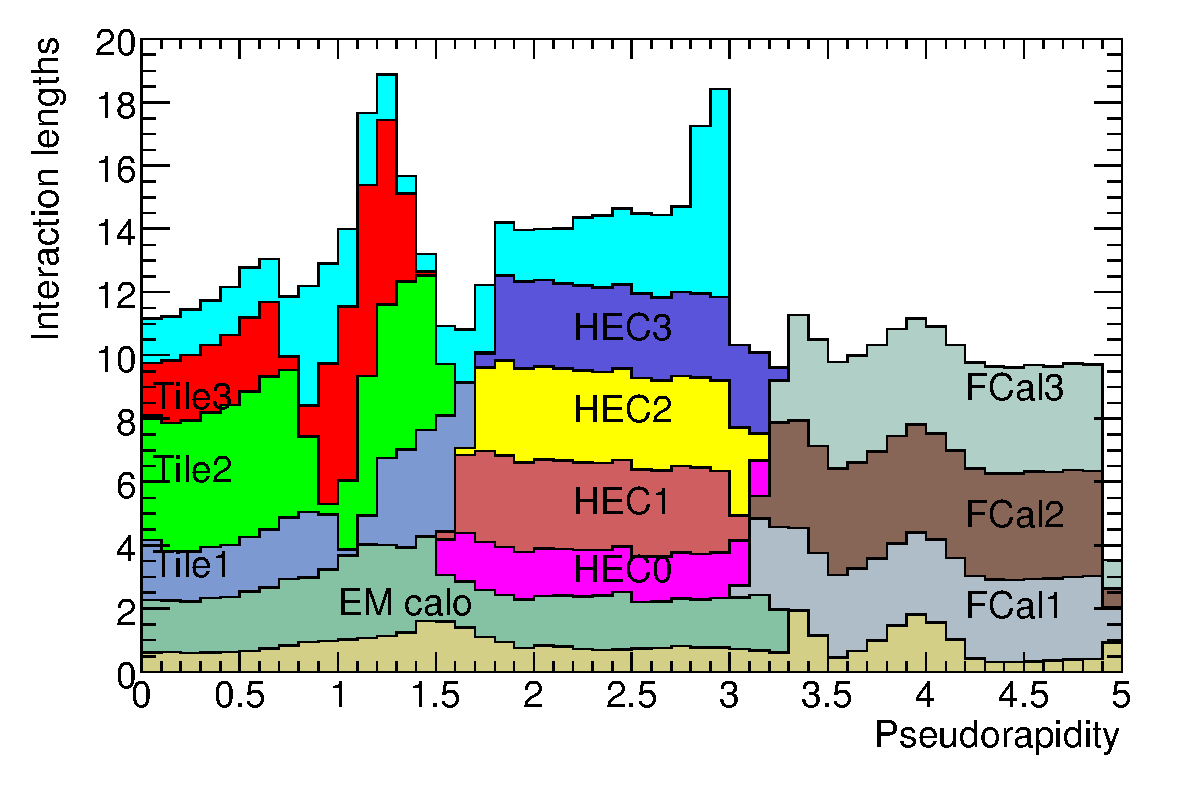
\includegraphics[width=\fullfig]{figures/calo_interactionlengths.pdf}
\caption{}
\label{fig:calo_interactionlengths}
\end{figure}

\begin{figure}[hbtp]
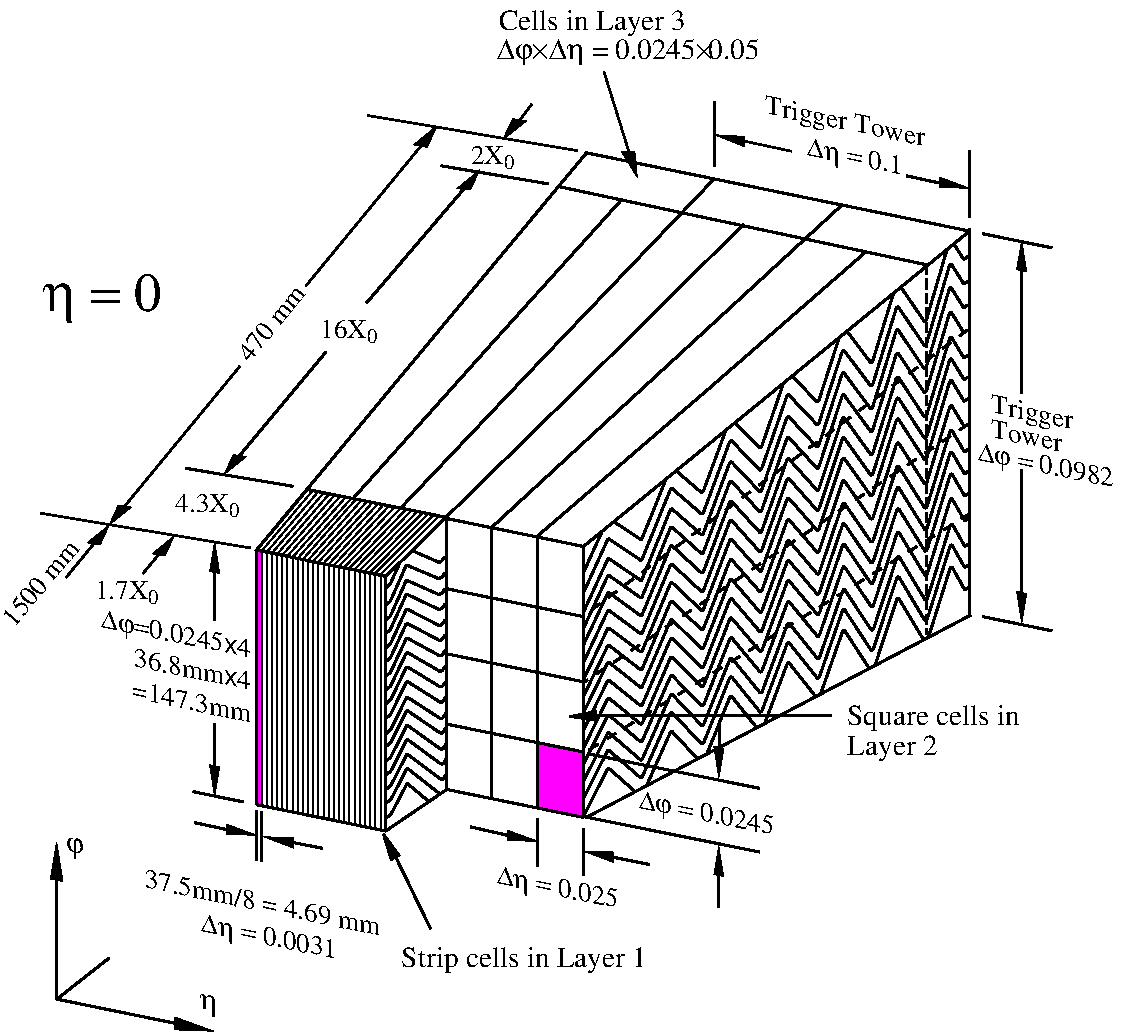
\includegraphics[width=\fullfig]{figures/calo_barrel_schematic.pdf}
\caption{}
\label{fig:calo_barrel_schematic}
\end{figure}

\begin{figure}[hbtp]
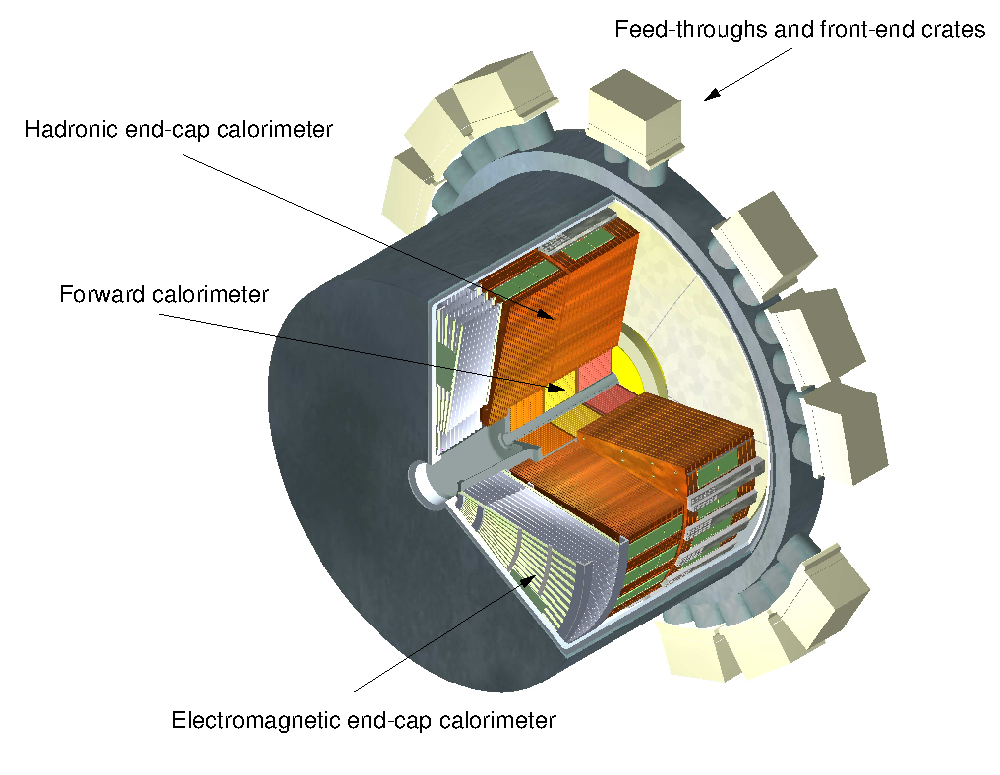
\includegraphics[width=\fullfig]{figures/calo_endcap_overview.pdf}
\caption{}
\label{fig:calo_endcap_overview}
\end{figure}


\subsection{Electromagnetic Calorimeters}

\begin{figure}[hbtp]
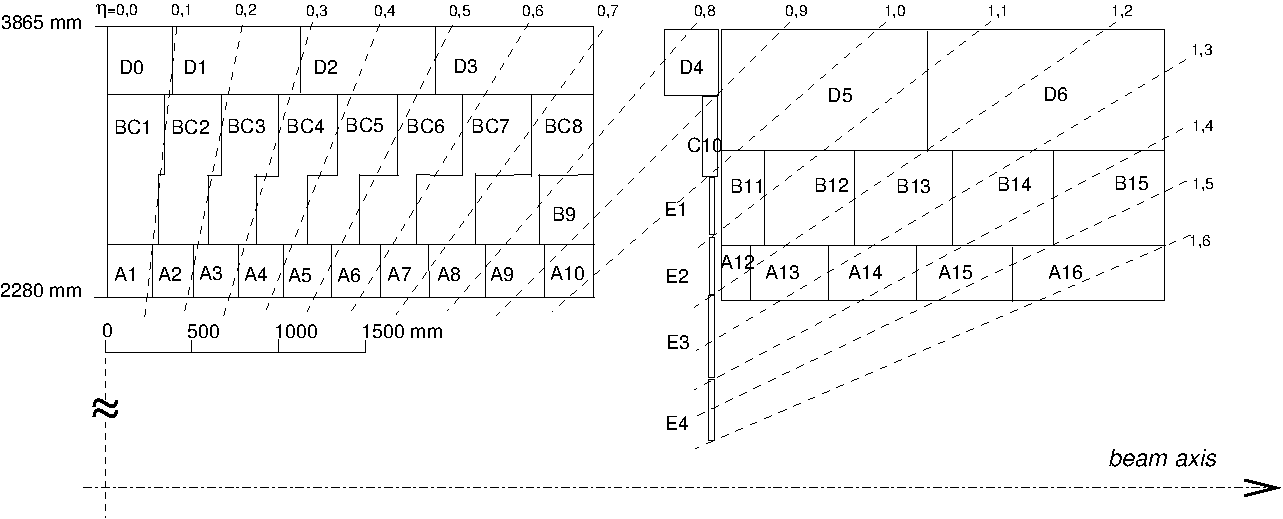
\includegraphics[width=\fullfig]{figures/tile_segmentation.pdf}
\caption{}
\label{fig:tile_segmentation}
\end{figure}


\subsection{Hadronic Calorimeters}

\subsection{Forward Calorimeters}

% ----------------------------------------

\section{Muon Spectrometer}

\begin{figure}[hbtp]
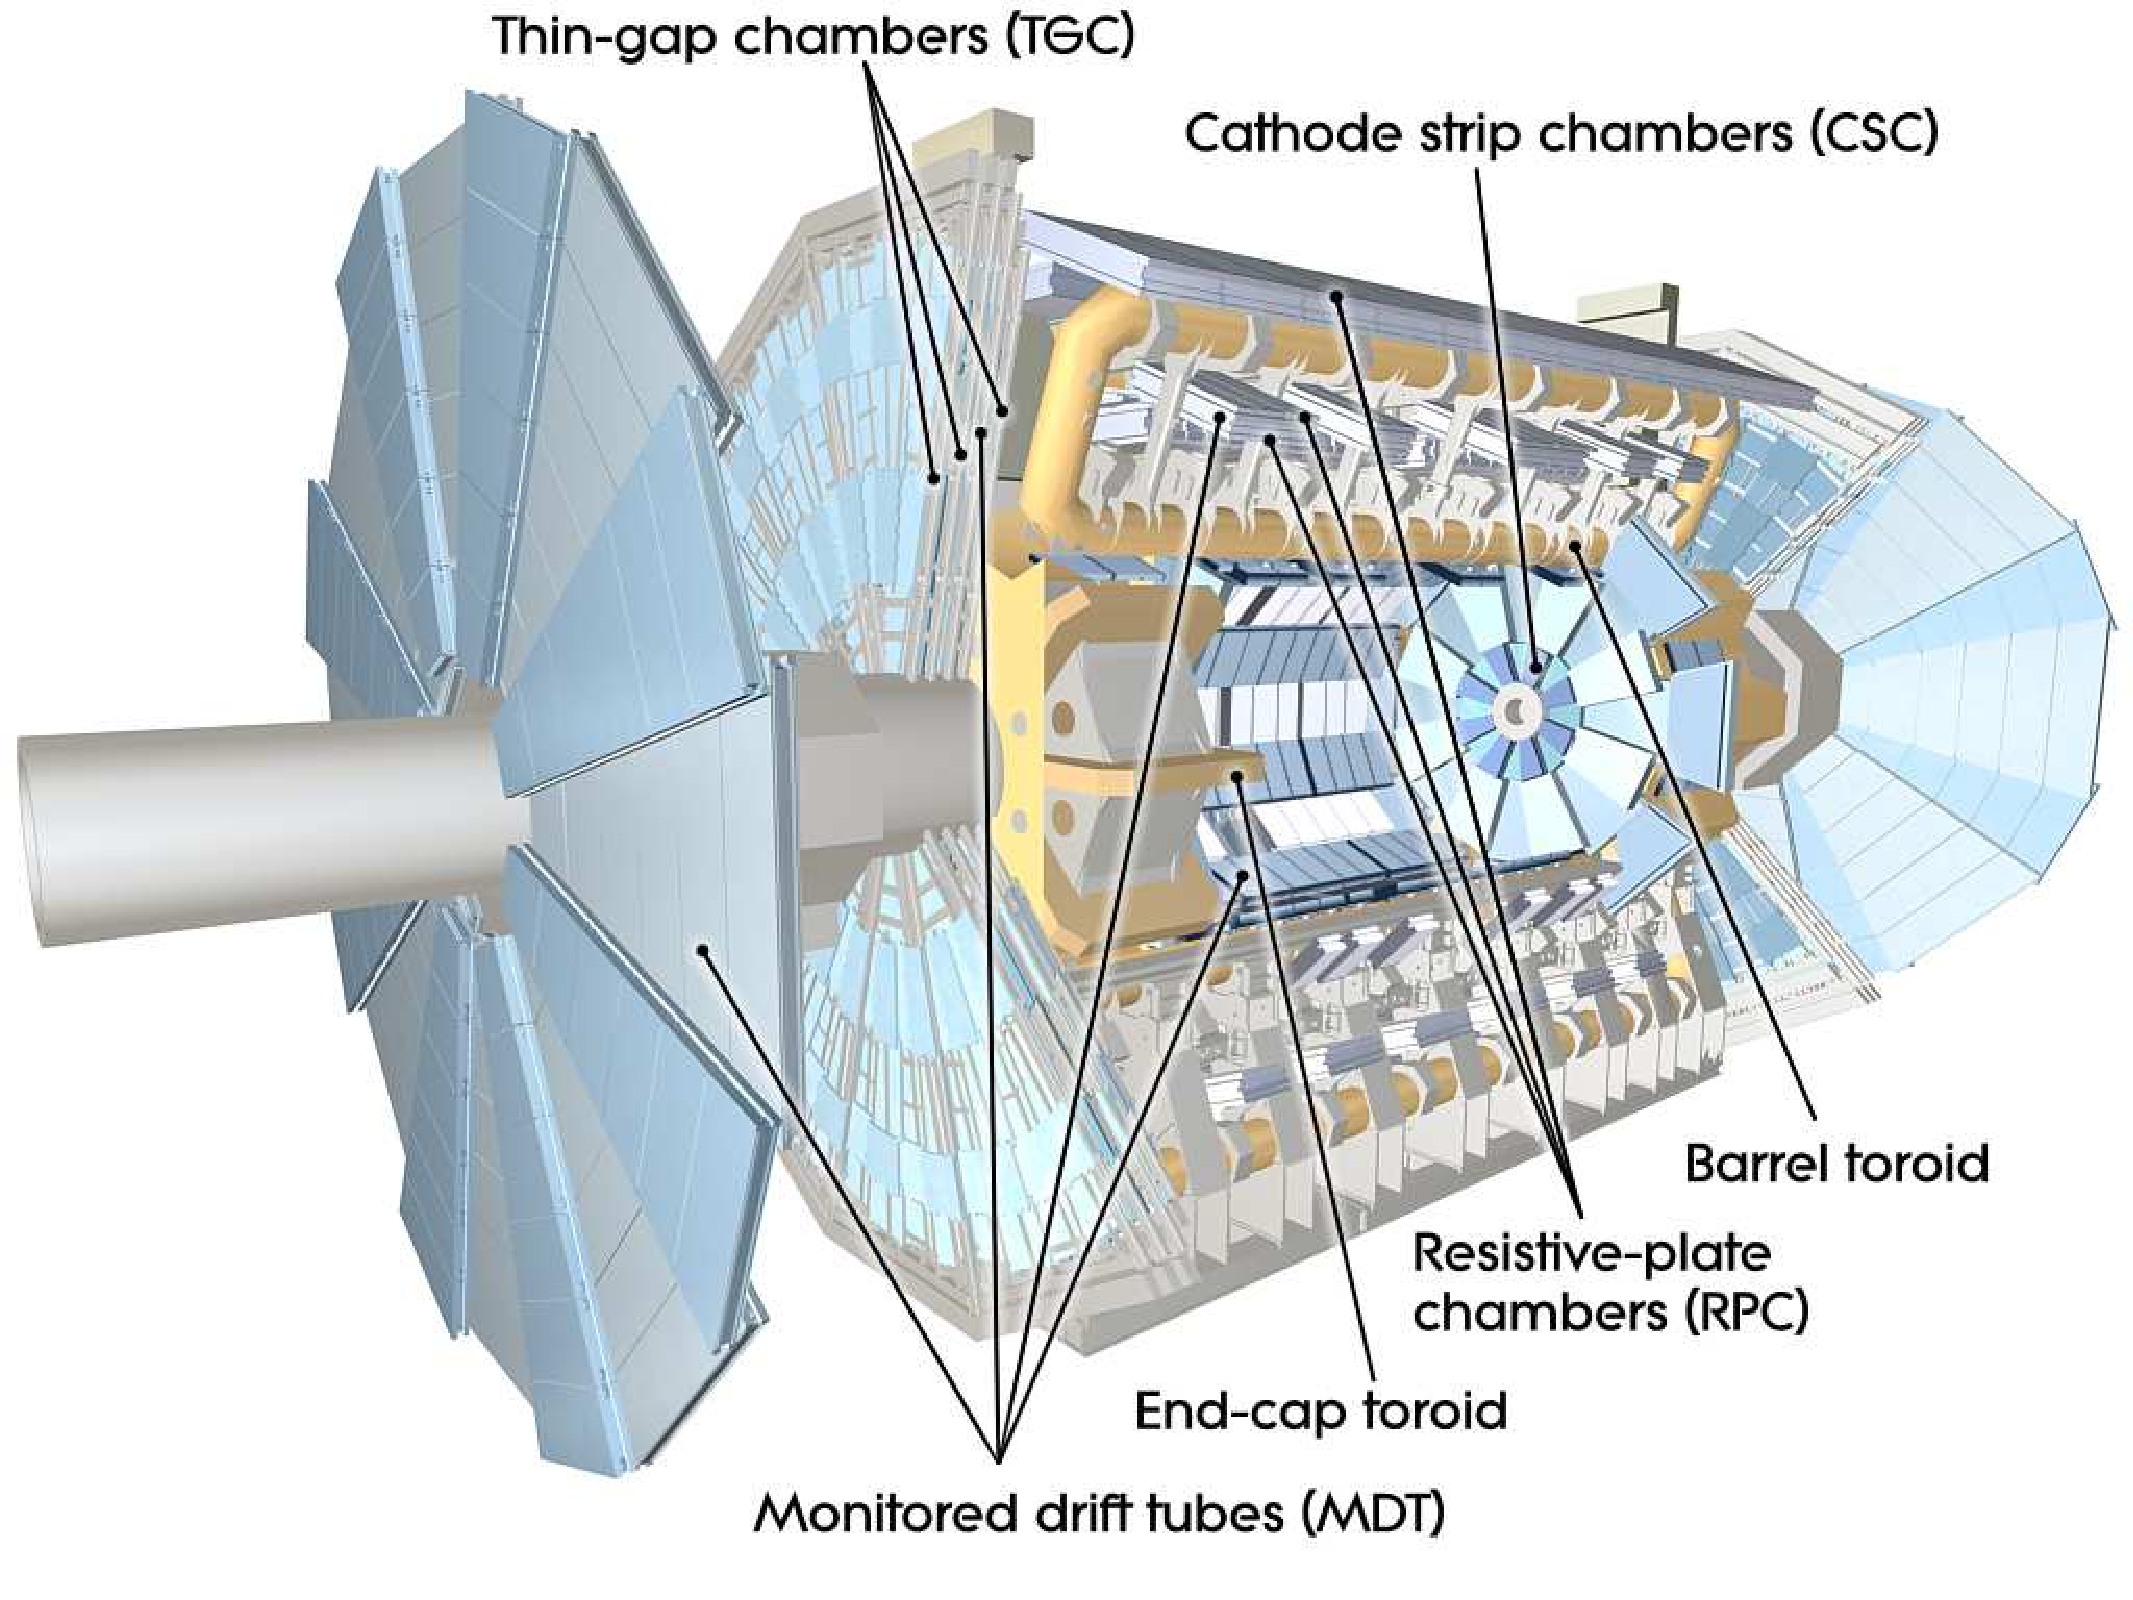
\includegraphics[width=\fullfig]{figures/muon_overview.pdf}
\caption{}
\label{fig:muon_overview}
\end{figure}


\begin{figure}[hbtp]
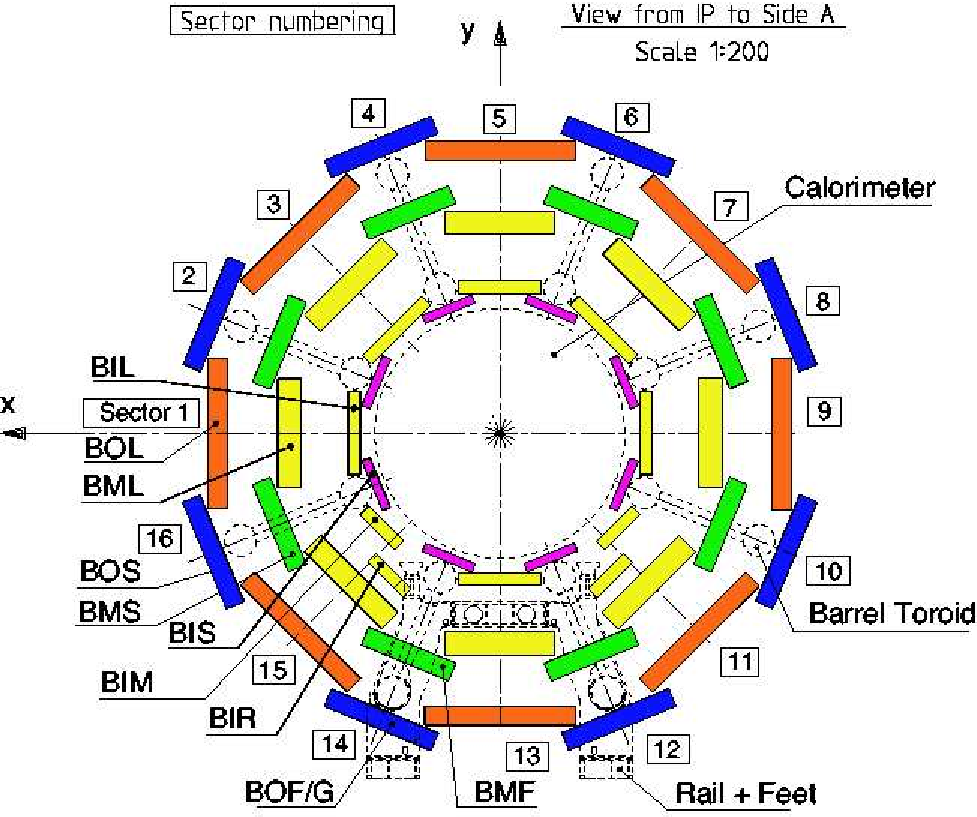
\includegraphics[width=\fullfig]{figures/muon_barrel_schematic.pdf}
\caption{}
\label{fig:muon_barrel_schematic}
\end{figure}

\begin{figure}[hbtp]
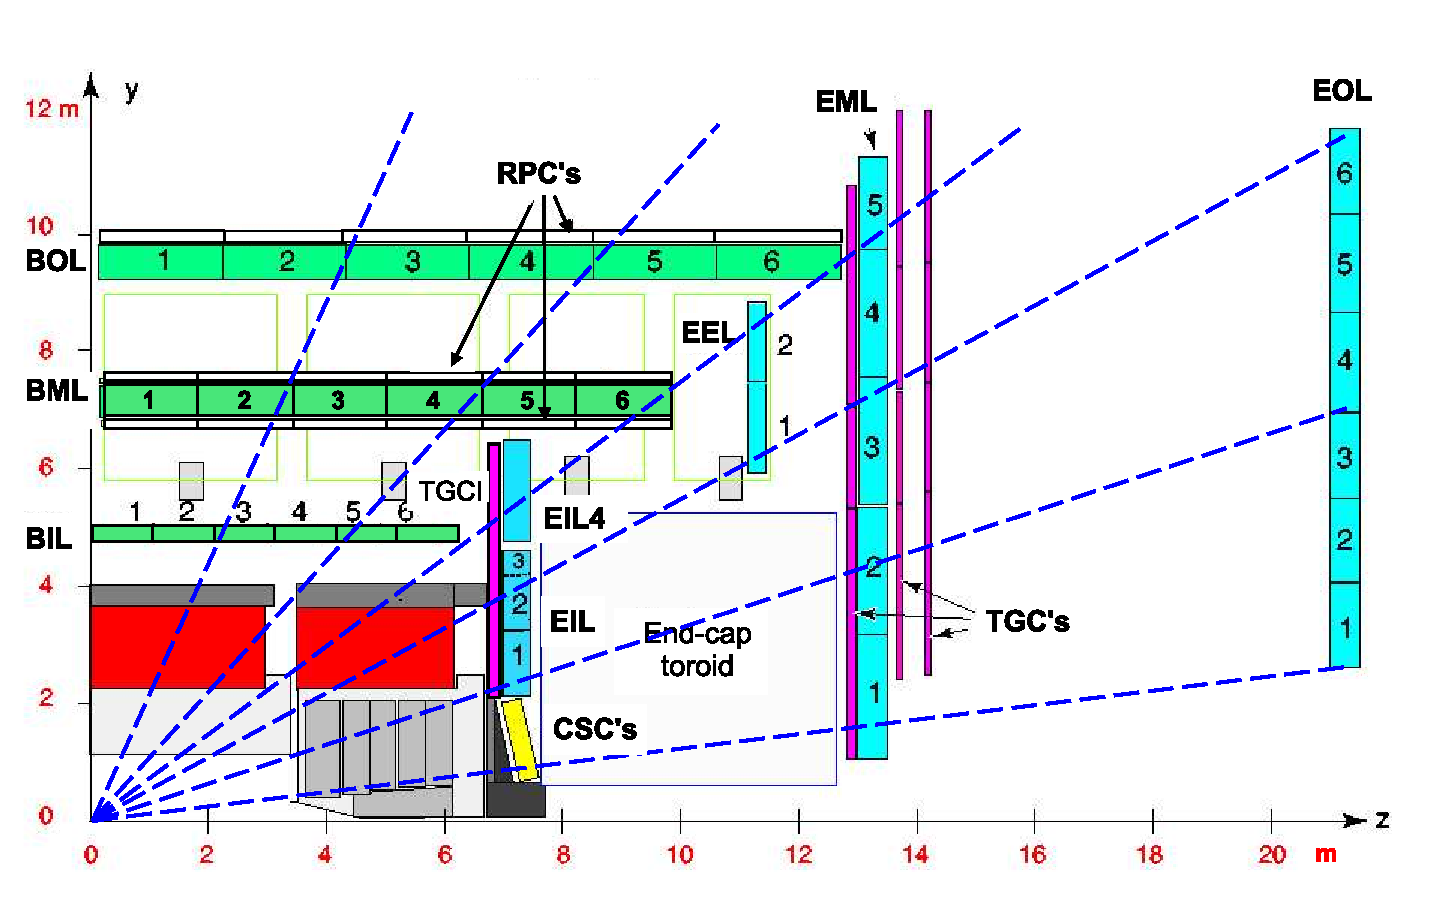
\includegraphics[width=\fullfig]{figures/muon_side_schematic.pdf}
\caption{}
\label{fig:muon_side_schematic}
\end{figure}


% ----------------------------------------

\section{Trigger}
\label{sec:trigger}

\subsection{Trigger Scheme}

\begin{figure}[hbtp]
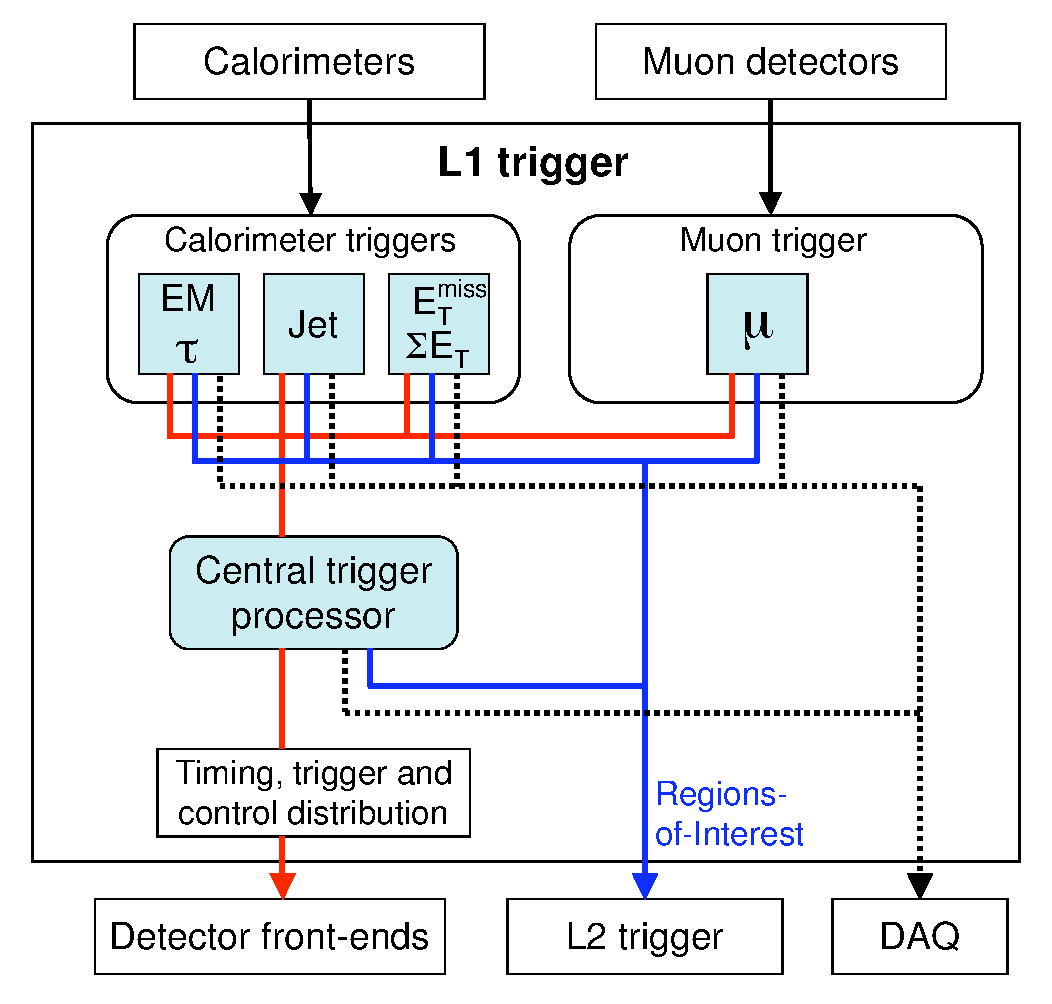
\includegraphics[width=\fullfig]{figures/l1_diagram.pdf}
\caption{}
\label{fig:l1_diagram}
\end{figure}

\subsection{Missing Transverse Energy Triggers}

% ----------------------------------------
